\documentclass[11pt]{article}
\usepackage[letterpaper,margin=0.9in]{geometry}
\ifdefined\XeTeXrevision\else\usepackage[T1]{fontenc}\fi
\usepackage{amsmath,amssymb,amsthm}
\usepackage{newtxtext,newtxmath}
\usepackage{graphicx}
\usepackage{booktabs}
\usepackage{array}
\usepackage[font=small,labelfont=bf]{caption}
\usepackage{microtype}
\usepackage{url}
\usepackage[colorlinks=true,linkcolor=blue,citecolor=blue,urlcolor=blue]{hyperref}

\newtheorem{theorem}{Theorem}
\newtheorem{lemma}{Lemma}[section]
\newtheorem{proposition}[lemma]{Proposition}
\newtheorem{corollary}[lemma]{Corollary}
\theoremstyle{remark}
\newtheorem{remark}[lemma]{Remark}
\numberwithin{equation}{section}

\newcommand{\Z}{\mathbb{Z}}
\newcommand{\R}{\mathbb{R}}
\newcommand{\C}{\mathbb{C}}
\newcommand{\T}{\mathbb{T}}
\newcommand{\E}{\mathbb{E}}
\newcommand{\Tr}{\operatorname{Tr}}
\newcommand{\spec}{\operatorname{spec}}
\renewcommand{\Re}{\operatorname{Re}}
\renewcommand{\Im}{\operatorname{Im}}
\newcommand{\Li}{\operatorname{Li}_2}
\newcommand{\Cl}{\operatorname{Cl}_2}
\newcommand{\IME}{I_{\mathrm{ME}}}
\newcommand{\FD}{F_{\mathrm{DKZ}}}
\newcommand{\one}{\mathbf{1}}
\newcommand{\ip}[2]{\langle #1,#2\rangle}
\newcommand{\cD}{\mathcal{D}}
\newcommand{\cN}{\mathcal{N}}
\newcommand{\cL}{\mathcal{L}}
\newcommand{\cE}{\mathcal{E}}
\newcommand{\Sh}{\Xi^{\sharp}}
\newcommand{\Phic}{\Phi_{\mathrm c}}
\newcommand{\lmin}{\lambda_{\min}}
\newcommand{\lmax}{\lambda_{\max}}
\newcommand{\dd}{\,\mathrm{d}}
\newcommand{\vc}{v_{\mathrm c}}
\newcommand{\veven}{v_{\mathrm{even}}}
\newcommand{\vodd}{v_{\mathrm{odd}}}
\newcommand{\CH}{\mathrm{CH}}
\newcommand{\DKZ}{\mathrm{DKZ}}
\newcommand{\CONE}{\mathrm{CONE}}
\newcommand{\UNI}{\mathrm{UNI}}
\newcommand{\UC}{\mathrm{UC}}
\newcommand{\COR}{\mathrm{COR}}
\newcommand{\sA}{\mathsf{A}}
\newcommand{\sB}{\mathsf{B}}
\setlength{\emergencystretch}{2em}
\renewcommand{\topfraction}{0.9}
\renewcommand{\textfraction}{0.1}
\renewcommand{\floatpagefraction}{0.8}
\makeatletter\@secpenalty=0\makeatother

\begin{document}

\begin{center}
{\LARGE\bfseries The power of CGLMP inequalities:\\[4pt]
completing the resolution of IQOQI Vienna\\[4pt] Open Quantum Problem~27\par}
\vspace{14pt}
{\large Ansh Mishra$^{1,\ast}$ and Aryan Senthilkumar$^{2}$\par}
\vspace{6pt}
{\small $^{1}$Independent researcher, Cumming, GA, USA\par
$^{2}$Independent researcher, Johns Creek, GA, USA\par
E-mail: \href{mailto:ansh.mishra2025@gmail.com}{ansh.mishra2025@gmail.com} (A.M.),
\href{mailto:aryan.senthilk@gmail.com}{aryan.senthilk@gmail.com} (A.S.)\par
$^\ast$Corresponding author\par
\vspace{6pt}
October 2026\par}
\end{center}

\begin{abstract}
\noindent Open Quantum Problem~27 of IQOQI Vienna, ``The power of CGLMP inequalities'', asks (A) whether every
nontrivial facet of the local polytope with two settings and $d$ outcomes per party is of CGLMP type, and (B) to show
that the Fourier-type measurements of Durt, Kaszlikowski and \.Zukowski (DKZ) are necessarily optimal for the CGLMP
inequality on a maximally entangled state, that they realize the highest resistance of the violation to noise, and
that they give the best Kullback--Leibler discrimination against local realism. Part~A was answered negatively by
Bancal, Gisin and Pironio in 2010. We settle every clause of Part~B as posed. (i)~For every $d$, every local dimension
and all projective measurements on maximally entangled states, the CGLMP value is at most the DKZ value, and DKZ is the
only maximizer up to local unitaries and an inert ancilla. The proof combines an exact reduction to a clock model, a new
strip inequality for a projection and a Hermitian matrix, obtained from a two-variable Bessis--Moussa--Villani
positivity theorem with an explicit density, and a cone condition on Clausen kernels certified in interval arithmetic
for every $d$; it is formalised in Lean~4, completely for $d\le20$ and, for $d\ge21$, up to the certified cone
condition. (ii)~The noise clause holds for every $d$ for the violation of the CGLMP inequality, with DKZ the unique
optimum; in Gill's literal reading (uniformly random outcomes as noise, violation of any Bell inequality) it fails for
every $d\ge4$ on the maximally entangled state of two $d$-level systems, by projective measurements of coarse-grained
CHSH type whose critical visibility we compute exactly. (iii)~The Kullback--Leibler clause fails for every $d\ge4$:
explicit orthonormal-basis measurements reach a statistical strength of at least $0.0703$ bits, DKZ at most $0.0688$
bits. Open strengthenings are listed.
\end{abstract}

%==============================================================================================================
\section{Introduction}\label{sec:intro}
%==============================================================================================================

\subsection{The problem}
The inequalities of Collins, Gisin, Linden, Massar and Popescu (CGLMP)~\cite{CGLMP} are Bell inequalities for two
parties who each choose one of two measurement settings and obtain one of $d$ outcomes. They define facets of the local
polytope of this scenario~\cite{Masanes}, they reduce to the inequality of Clauser, Horne, Shimony and Holt
(CHSH)~\cite{CHSH} for $d=2$, and they are the standard tool for certifying nonlocality with high-dimensional systems.
Open Quantum Problem~27 of IQOQI Vienna, ``The power of CGLMP inequalities''~\cite{OQP}, proposed by R.~Gill in 2006,
asks how special these inequalities and their optimal quantum measurements are. It has two parts.

\emph{Part~A} asks to prove that every face of the local polytope that does not already lie in a face of the
no-signalling polytope is of CGLMP type: it is the inequality written out in~\cite{CGLMP}, or a lifting of it from
fewer outcomes, obtained by fusing outcomes.

\emph{Part~B} starts from the numerical observation~\cite{DKZ} that the observables maximizing the CGLMP violation on
a maximally entangled state take a very special form, namely computational-basis measurements preceded by a discrete
Fourier transform and diagonal unitaries~\cite{CGLMP}. It asks to prove (i)~that this must be so, (ii)~that these
measurements have the largest resistance of the violation to noise, and (iii)~that they discriminate best against
classical realism in the Kullback--Leibler sense~\cite{vDGG}.

The exact wording is on the archived problem page~\cite{OQP} and in the clause-by-clause ledger of the accompanying
repository~\cite{repo} (file \texttt{complete-resolution/LEDGER.md}). We label the clauses 27A, 27B(i), 27B(ii) and
27B(iii). The problem goes back to Gill's paper~\cite{Gill}, in which the resistance of a violation to noise is measured
by how much of the distribution of ``completely random, uniform outcomes''~\cite[p.~140]{Gill} can be mixed into the
observed one while local realism is still violated. The measurements of Part~B were found numerically by Kaszlikowski
et al.~\cite{KGZMZ} and described analytically by Durt, Kaszlikowski and \.Zukowski~\cite{DKZ}; we call them the
\emph{DKZ measurements}. Each party applies setting-dependent diagonal phases, then a discrete Fourier transform, and
measures in the computational basis.

\subsection{Previous work}
Part~A was answered negatively by Bancal, Gisin and Pironio~\cite{BGP}: for $d=4$ the local polytope has facets that
are not of CGLMP type. For 27B(i), the optimality of the DKZ value $\IME(d)$ of~\eqref{eq:IME} is Tsirelson's
bound~\cite{Tsirelson} for $d=2$; for $d=3$ a semidefinite relaxation agrees with it to within $10^{-10}$~\cite{LVN}
(the partial result listed on the problem page); and in earlier work we proved optimality and uniqueness for
$3\le d\le20$ by exact sum-of-squares certificates~\cite{repoCGLMP}, and for every $d$ for the strategies whose four
``link'' operators coincide~\cite{MSclassical}. Over all states the largest CGLMP value is attained by states that are
not maximally entangled for $d\ge3$~\cite{ADGL}, and it is known exactly only for $d\le8$~\cite{IR,repoCGLMP}. For
27B(ii), the critical visibilities of the DKZ measurements were computed numerically~\cite{KGZMZ,DKZ} and identified
with the CGLMP threshold $2/\IME(d)$~\cite[eq.~(23)]{CGLMP}; see also~\cite{Chen01} ($d=3$) and~\cite{GLZ} ($d\le5$,
where states of Schmidt rank two are the most noise-robust). Ac\'{\i}n, Durt, Gisin and Latorre~\cite[eq.~(14)]{ADGL}
showed that the CHSH strategy on a maximally entangled state of Schmidt rank two in $\C^d\otimes\C^d$ has a critical
visibility tending to $0$, and Baek, Ryu and Lee~\cite{BRL} observed numerically that merging outcomes increases the
noise robustness of the optimal CGLMP correlations on $\Phi_4$ and $\Phi_{16}$. For 27B(iii), van Dam, Gill and
Gr\"unwald~\cite{vDGG} introduced the statistical strength of a nonlocality proof; Ac\'{\i}n, Gill and Gisin~\cite{AGG}
showed that the best tests need not use maximally entangled states; Zhang~\cite{Zhang} found the first counterexample to
the clause ($d=4$, with an exact certificate); and we gave counterexamples for $4\le d\le9$~\cite{repoCGLMP}.

\subsection{Results}
This paper settles every clause of Part~B as originally posed, so that every clause of Problem~27 now has a verdict
(Table~\ref{tab:status}); the verdict on the noise clause depends on its reading.

\emph{(i)} For every $d\ge2$, every local dimension $D$ and all projective measurements on $\Phi_D$, $I_d\le\IME(d)$,
and the DKZ measurements are the only maximizers up to a local unitary $u\otimes\bar u$ and an inert auxiliary system
(Theorems~\ref{thm:opt} and~\ref{thm:rig}); for $3\le d\le8$ this extends to arbitrary POVMs
(Proposition~\ref{prop:povm}). The proof combines an exact reduction to $4d$ projections on a circle, a new strip
inequality for a projection and a Hermitian matrix (Theorem~\ref{thm:strip}), proved through a two-variable positivity
theorem of Bessis--Moussa--Villani type with an explicit density (Theorem~\ref{thm:bmv}), a noncommutative continuum
theorem, and a cone condition on Clausen kernels (Theorem~\ref{thm:cone}) certified in interval arithmetic for every $d$;
it is formalised in Lean~4, completely for $2\le d\le20$ and, for $d\ge21$, up to the cone condition.

\emph{(ii)} For the violation of the CGLMP inequality, the noise clause holds for every $d$, with DKZ the unique optimum
(Theorem~\ref{thm:noisecglmp}). In Gill's literal reading (uniformly random outcomes as noise, violation of local
realism) it fails for every $d\ge4$ on $\Phi_d$ itself: projective measurements of coarse-grained CHSH type, with unused
outcomes, have an exactly computed critical visibility below that of DKZ, which is at least $\frac12$
(Theorem~\ref{thm:literal}). It holds for $d=2$, and for $d=3$ it holds on $\Phi_3$ and fails on $\Phi_2$
(Proposition~\ref{prop:small}).

\emph{(iii)} The Kullback--Leibler clause fails for every $d\ge4$, for all three strengths of~\cite{vDGG}: explicit
orthonormal-basis measurements on $\Phi_d$ reach at least $0.0703203$ bits, DKZ at most $0.0687803$ bits
(Theorem~\ref{thm:kl}); for $d=3$, DKZ is a strict local maximum (Proposition~\ref{prop:kl3}).

As far as we found, the following are new: Theorems~\ref{thm:opt} and~\ref{thm:rig} for $d\ge21$ (for $3\le d\le20$
see~\cite{repoCGLMP}); Theorem~\ref{thm:strip}; the exact theorem on Gill's literal noise clause for every $d\ge4$ and
its consequence for Problem~27 (the mechanism is that of~\cite{ADGL}); and the failure of the Kullback--Leibler clause
for every $d\ge4$ ($d=4$ first in~\cite{Zhang}). Theorem~\ref{thm:bmv} uses the Fourier-slice mechanism of
Hein\"avaara~\cite{He}, for which we claim no novelty. Questions beyond the problem as posed remain open
(Section~\ref{sec:open}).

\begin{table}[t]
\centering\small
\caption{The clauses of Open Quantum Problem~27 as originally posed~\cite{OQP}, and their status. The positive results
concern projective measurements (27B(i) also holds for POVMs when $3\le d\le8$, Proposition~\ref{prop:povm}); the
counterexamples use projective measurements. Lean: Section~\ref{subsec:lean}.}
\label{tab:status}
\begin{tabular}{@{}>{\raggedright\arraybackslash}p{0.31\textwidth}>{\raggedright\arraybackslash}p{0.33\textwidth}>{\raggedright\arraybackslash}p{0.30\textwidth}@{}}
\toprule
Clause & Verdict & Proof; credit\\
\midrule
27A: every face of the local polytope not contained in a face of the no-signalling polytope is of CGLMP type,
possibly lifted & \textbf{false}: non-CGLMP facets for $d=4$ & Bancal, Gisin and Pironio~\cite{BGP} (prior work)\\
27B(i): the DKZ measurements are necessarily the optimal ones on maximally entangled states & \textbf{true for every
$d$}: optimal, and unique up to $u\otimes\bar u$ and an inert ancilla (any local dimension) &
Theorems~\ref{thm:opt},~\ref{thm:rig} (this work); Lean-verified for $d\le20$, and for $d\ge21$ given $\CONE_d$;
earlier: $d=2$~\cite{Tsirelson}, $3\le d\le20$~\cite{repoCGLMP}, commuting strategies~\cite{MSclassical}\\
27B(ii), CGLMP reading: resistance of the CGLMP violation to uniform noise & \textbf{true for every $d$}; DKZ the
unique optimum & Theorem~\ref{thm:noisecglmp} (this work); Lean-verified with the same scope\\
27B(ii), Gill's literal reading: violation of local realism under uniform outcome noise & \textbf{false for every
$d\ge4$}, on $\Phi_d$ itself; true for $d=2$; $d=3$: true on $\Phi_3$, false on $\Phi_2$ &
Theorem~\ref{thm:literal}, Proposition~\ref{prop:small} (this work); mechanism~\cite[eq.~(14)]{ADGL}; numerics for
$d=4,16$~\cite{BRL}\\
27B(iii): best Kullback--Leibler discrimination & \textbf{false for every $d\ge4$} (all three strengths
of~\cite{vDGG}); $d=3$: DKZ a strict local maximum & Theorem~\ref{thm:kl}, Proposition~\ref{prop:kl3} (this work);
$d=4$ first by Zhang~\cite{Zhang}; $4\le d\le9$~\cite{repoCGLMP}\\
\bottomrule
\end{tabular}
\end{table}

\paragraph{Organisation.}
Section~\ref{sec:27Bi} states and outlines the proof of 27B(i), with complete proofs in the companion
paper~\cite{MSmath} (see also~\cite{MSoverview}); Sections~\ref{sec:noise} and~\ref{sec:kl} prove the noise and
Kullback--Leibler verdicts; Section~\ref{sec:verification} covers verification and Section~\ref{sec:open} open questions.

%==============================================================================================================
\section{Setting and notation}\label{sec:setting}
%==============================================================================================================

\paragraph{Behaviours and local models.}
The settings are $x,y\in\{1,2\}$ and the outcomes $a,b\in\Z_d=\{0,\dots,d-1\}$. A \emph{behaviour}
$p=(p(\cdot,\cdot|x,y))_{x,y}$ is a family of four probability distributions on $\Z_d\times\Z_d$. For
$\lambda=(a_1,a_2,b_1,b_2)\in\Z_d^4$ let $\delta_\lambda(a,b|x,y)=[a=a_x][b=b_y]$ ($[\cdot]$ is the Iverson bracket).
The \emph{local polytope} is $\cL_d=\operatorname{conv}\{\delta_\lambda:\lambda\in\Z_d^4\}$; a behaviour in $\cL_d$ is
\emph{local}, and a probability distribution on $\Z_d^4$ is a \emph{local model} (local randomness of the parties can
be absorbed into it). Relabellings of settings, of the outcomes of each measurement and of the parties, and local
post-processings of the outcomes, map $\cL_d$ into itself. We write $p_0(a,b|x,y)=d^{-2}$ for the behaviour of
completely random, uniform outcomes; it is local.

\paragraph{The CGLMP expression.}
Write $P(A_x=B_y+k)$ for the probability that $A_x-B_y\equiv k\pmod d$ for the settings $x,y$. The CGLMP expression is
\begin{multline}\label{eq:cglmp}
I_d=\sum_{k=0}^{\lfloor d/2\rfloor-1}\Bigl(1-\frac{2k}{d-1}\Bigr)\Bigl(\bigl[P(A_1=B_1+k)+P(B_1=A_2+k+1)
+P(A_2=B_2+k)+P(B_2=A_1+k)\bigr]\\
-\bigl[P(A_1=B_1-k-1)+P(B_1=A_2-k)+P(A_2=B_2-k-1)+P(B_2=A_1-k-1)\bigr]\Bigr),
\end{multline}
the reading of~\cite{CGLMP} under which the local bound is derived and the DKZ measurements give $\IME(d)$
(see~\cite[Section~2]{MSclassical}). Local behaviours satisfy $I_d\le2$~\cite{CGLMP}, and $I_d(p_0)=0$, since every
probability in~\eqref{eq:cglmp} equals $1/d$ under $p_0$ and each term has four of them with each sign. For $d=2$,
$I_2$ is the CHSH expression.

\paragraph{Projective strategies on maximally entangled states.}
Such a strategy consists of a local dimension $D\ge1$, the state $\Phi_D=D^{-1/2}\sum_{i=1}^D|ii\rangle$, and
projection-valued measures $\{P^x_a\}_{a\in\Z_d}$ (Alice) and $\{Q^y_b\}_{b\in\Z_d}$ (Bob) on $\C^D$, zero projections
allowed. Its behaviour is $p(a,b|x,y)=\langle\Phi_D|P^x_a\otimes Q^y_b|\Phi_D\rangle=\frac1D\Tr\bigl((P^x_a)^{\mathsf
T}Q^y_b\bigr)$, the transpose being taken in the Schmidt basis. Local unitaries $u\otimes\bar u$ fix $\Phi_D$, and
tensoring a strategy with the identity on an inert auxiliary system, on $\Phi_{Dk}=\Phi_D\otimes\Phi_k$, does not change
its behaviour.

\paragraph{The DKZ strategy.}
The DKZ strategy $\DKZ_d$ ($D=d$) measures in the bases
\[
|k\rangle_{A,x}=d^{-1/2}\sum_je^{-2\pi ij(k+\alpha_x)/d}|j\rangle,\qquad|l\rangle_{B,y}=d^{-1/2}\sum_je^{2\pi ij(l-\beta_y)/d}|j\rangle,
\qquad\alpha=(0,\tfrac12),\quad\beta=(\tfrac14,-\tfrac14)
\]
(the measurements of~\cite[eqs.~(12)--(15)]{CGLMP}). Since
$|\sum_{j<d}e^{2\pi ij\theta/d}|^2=\sin^2(\pi\theta)/\sin^2(\pi\theta/d)$,
\begin{equation}\label{eq:dkzclosed}
p_{\DKZ}(a,b|x,y)=\frac1d\,h_{xy}(b-a),\qquad h_{xy}(m)=\frac1{2d^2\sin^2\bigl(\pi(m-\delta_{xy})/d\bigr)},
\end{equation}
with $\delta_{xy}=\alpha_x+\beta_y$, that is, $\delta_{11}=\delta_{22}=\frac14$, $\delta_{12}=-\frac14$, $\delta_{21}=\frac34$;
each $h_{xy}$ is a probability distribution on $\Z_d$, so $p_{\DKZ}$ has uniform marginals. The DKZ value
is~\cite{DKZ,CGLMP}
\begin{equation}\label{eq:IME}
\IME(d)=I_d(p_{\DKZ})=\frac{4}{d(d-1)}\sum_{j=1}^{d-1}(d-j)\sec\frac{\pi j}{2d},
\end{equation}
for instance $\IME(2)=2\sqrt2$, $\IME(3)=(12+8\sqrt3)/9=2.8729\ldots$, $\IME(4)=2.8962\ldots$, $\IME(20)=2.9547\ldots$, and
$\IME(d)\to32G/\pi^2=2.9698\ldots$ as $d\to\infty$, where $G$ is Catalan's constant (Remark~\ref{rem:limit}).

\paragraph{Noise.}
For a behaviour $p$ and $0\le v\le1$ put $p_v=vp+(1-v)p_0$ and $\vc(p)=\max\{v\in[0,1]:p_v\in\cL_d\}$, the
\emph{critical visibility}; $p_v$ is local exactly for $v\le\vc(p)$, and a \emph{smaller} $\vc$ means a \emph{higher}
resistance to noise. Relabellings fix $\cL_d$ and $p_0$, hence $\vc$. For a strategy we write $\vc$ of its behaviour.

\paragraph{Conventions.}
$\tau=\frac1M\Tr$ is the normalised trace on $M_M(\C)$, $X_+$ the positive part of a Hermitian $X$, $\|\cdot\|_F$ the
Frobenius norm, and $\Tr_Ef(EXE)$ the trace over $\operatorname{ran}E$ of $f$ of the compression of $X$ by a projection
$E$; $\Cl(\theta)=\sum_{n\ge1}n^{-2}\sin n\theta$ is the Clausen function and $G=\Cl(\pi/2)$ Catalan's constant.
\emph{Computer-assisted} means: depending on computations in rigorous interval arithmetic with outward rounding, or in
exact rational or algebraic arithmetic; floating-point computations only find certificates and never decide a statement.

%==============================================================================================================
\section{Clause 27B(i): the DKZ measurements are optimal and unique}\label{sec:27Bi}
%==============================================================================================================

\subsection{Statements}\label{subsec:statements}

\begin{theorem}[optimality; computer-assisted]\label{thm:opt}
Let $d\ge2$ and $D\ge1$. For every projective strategy on the maximally entangled state $\Phi_D$, $I_d\le\IME(d)$. The
DKZ strategy attains $\IME(d)$.
\end{theorem}

\begin{theorem}[rigidity; computer-assisted]\label{thm:rig}
Let $d\ge2$, $D\ge1$, and suppose that a projective strategy on $\Phi_D$ attains $I_d=\IME(d)$. Then $d$ divides $D$,
and there is a unitary $u\colon\C^D\to\C^d\otimes\C^{D/d}$ such that $uP^x_au^*=P^{x,\DKZ}_a\otimes\one$ and
$\bar uQ^y_b\bar u^{\,*}=Q^{y,\DKZ}_b\otimes\one$ for all $x,y,a,b$. Moreover $(u\otimes\bar u)\Phi_D=\Phi_d\otimes\Phi_{D/d}$,
and $u$ is unique up to $u\mapsto(\one_d\otimes u')u$ with $u'$ unitary. Consequently, if $d\nmid D$, the maximum of
$I_d$ over projective strategies on $\Phi_D$ is strictly smaller than $\IME(d)$.
\end{theorem}

Theorems~\ref{thm:opt} and~\ref{thm:rig} are Theorems~A and~B of the companion mathematical paper~\cite{MSmath}, which
proves every statement of this section in full. They are computer-assisted only through Theorem~\ref{thm:cone} below
(interval arithmetic); for $2\le d\le20$ the whole proof, including Theorem~\ref{thm:cone}, is checked in Lean
(Section~\ref{subsec:lean}). They concern projective measurements, our reading of the observables of the problem; for
$3\le d\le8$ they extend to arbitrary POVMs (Proposition~\ref{prop:povm}), and for $d\ge9$ the POVM case is open
(Section~\ref{sec:open}).

The analytic core is an inequality for a projection and a Hermitian matrix of arbitrary size. Let
$S=\{z\in\C:0<\Re z<1\}$, and for $\lambda\in\R$, $z=x+iy\in S$ and $u\in\R$ put
\begin{equation}\label{eq:hK}
h_\lambda(x+iy)=-\frac1{\pi^2}\Im\Li\bigl(e^{\pi(y-\lambda)}e^{-i\pi x}\bigr),\qquad
K_x(u)=\frac{\sin\pi x}{2(\cosh\pi u-\cos\pi x)},
\end{equation}
with $\Li$ the dilogarithm (principal branch). $K_x$ is the Poisson kernel of $S$ for its left edge, and $h_\lambda$ is
the harmonic function on $S$ with boundary values $(y-\lambda)_+$ on $\Re z=0$ and $0$ on $\Re z=1$:
$h_\lambda(x+iy)=\int_\R(w-\lambda)_+K_x(y-w)\dd w$~\cite[Lemmas~3.1 and~3.2]{MSmath}.

\begin{theorem}[strip inequality]\label{thm:strip}
Let $B$ be an orthogonal projection on $\C^M$, $P=\one-B$, and $g$ a Hermitian $M\times M$ matrix. For every
$\lambda\in\R$,
\begin{equation}\label{eq:strip}
\sum_{\nu\in\spec(B+ig)}h_\lambda(\nu)-\Tr\bigl[(P(g-\lambda)P)_+\bigr]
=\int_0^1\!\!\int_\R K_{1-\tau}(s-\lambda)\,\rho(s,\tau)\dd s\dd\tau\;\ge\;0,
\end{equation}
where eigenvalues are counted with algebraic multiplicity and $\rho\ge0$ is the density of Theorem~\ref{thm:bmv}.
Equality holds for one $\lambda$ if and only if it holds for all $\lambda$, if and only if $Bg=gB$.
\end{theorem}

If $B$ and $g$ commute, the eigenvalues of $B+ig$ lie on the edges of $S$ and~\eqref{eq:strip} is an identity;
moving them into the strip by a non-commuting $g$ can only increase the left side.

\begin{theorem}[two-variable BMV positivity for projections]\label{thm:bmv}
In the situation of Theorem~\ref{thm:strip} let $\lmin\le\lmax$ be the extreme eigenvalues of $g$, and for $s\in\R$ and
$0<\tau<1$ let $\xi_1(s,\tau),\dots,\xi_M(s,\tau)$ be the roots, with multiplicity, of the polynomial
$\xi\mapsto\det\bigl(g-s-\xi(P-\tau)\bigr)$ of degree $M$. Put $\rho(s,\tau)=\frac1{2\pi}\sum_{i=1}^M|\Im\xi_i(s,\tau)|$
for $0<\tau<1$, and $\rho=0$ otherwise. Then $\rho$ is continuous on $\R\times(0,1)$, vanishes unless $\lmin<s<\lmax$,
satisfies $\rho(s,\tau)\le\frac M{2\pi}\|g-s\|(\tau(1-\tau))^{-1/2}$, and for all $(a,t)\in\C^2$
\begin{equation}\label{eq:bmv}
\cD(a,t):=\Tr e^{ag-tP}-e^{-t}\Tr_Pe^{aPgP}-\Tr_Be^{aBgB}=a^2\int_0^1\!\!\int_\R e^{as-t\tau}\rho(s,\tau)\dd s\dd\tau .
\end{equation}
Moreover $\int_\R\rho(s,\tau)\dd s=\|BgP\|_F^2$ for every $\tau\in(0,1)$.
\end{theorem}

At $a=1$, \eqref{eq:bmv} says that $t\mapsto\Tr e^{g-tP}$ is the Laplace transform of the positive measure
$\Tr_B(e^{BgB})\delta_0+\Tr_P(e^{PgP})\delta_1+(\int e^s\rho(s,\tau)\dd s)\dd\tau$ on $[0,1]$: Stahl's
theorem~\cite{Stahl} (the former Bessis--Moussa--Villani conjecture~\cite{BMV}) for a projection, with an explicit
density. Theorem~\ref{thm:bmv} asserts positivity in two variables after the pinched terms are subtracted and the result
is divided by $a^2$, and neither modification can be omitted. The mechanism of the proof (a Fourier transform of a
trace function of a pencil, computed along lines, with the density given by the imaginary parts of the roots of an
auxiliary pencil) was introduced by Hein\"avaara~\cite{He} for tracial joint spectral measures, giving a new proof of
Stahl's theorem (see also~\cite{Eremenko,LS}); Theorem~\ref{thm:bmv} is a variant adapted to a projection and an affine
chart, which we found independently, and we claim no novelty for the mechanism. We have not found
Theorem~\ref{thm:strip}, or an equivalent statement, in the literature; its continuum consequence
(Proposition~\ref{prop:continuum}) contains the circle version of the Stein--Weiss theorem~\cite{SW} on the conjugate
function of an indicator, in the form of Laeng~\cite{Laeng}.

The last ingredient involves only explicit special functions. Let $N=4d$, $\Xi(u)=-\frac{N^2}{2\pi^2}\Cl(\frac{2\pi
u}N)$ and $\Sh(u)=\Xi(u)+\Xi(2d-u)$ for $0\le u\le2d$, so that $(\Sh)''(u)=2\csc\frac{\pi u}{2d}$ on $(0,2d)$. Let
$\Delta_d=\{\ell\in\R^d:\ell_r\ge0,\ \sum_r\ell_r=d\}$ (the \emph{cell vectors}) and $\Delta_d^+$ its interior
($\ell_r>0$ for all $r$). For $\ell\in\Delta_d$, extended $d$-periodically, let $S_r(m)=\ell_r+\dots+\ell_{r+m-1}$ and
\begin{equation}\label{eq:uell}
u^\ell_m=\Delta^2_m\Bigl[\frac1d\sum_{r=0}^{d-1}\Sh\bigl(S_r(m)\bigr)\Bigr]\qquad(1\le m\le d-1),
\end{equation}
where $\Delta^2_mf=f(m+1)-2f(m)+f(m-1)$. Let $v\in\R^{d-1}$, $v_m=2\csc\frac{\pi m}{2d}$, and $t_s=e_s+e_{d-s}$.

\begin{theorem}[the cone condition $\CONE_d$; computer-assisted]\label{thm:cone}
For every $d\ge2$ there are a finite positive Borel measure $\mu$ on $\Delta_d$ with $\mu(\Delta_d^+)=\mu(\Delta_d)>0$
and numbers $w_s\ge0$ such that
\begin{equation}\label{eq:cone}
v=\int_{\Delta_d}u^\ell\,\mu(\dd\ell)+\sum_{s=1}^{\lfloor d/2\rfloor}w_s\,t_s .
\end{equation}
\end{theorem}

Theorems~\ref{thm:strip}, \ref{thm:bmv} and~\ref{thm:cone} are Theorems~C, D and~E of~\cite{MSmath}.

\subsection{Architecture of the proof}\label{subsec:architecture}

\begin{figure}[t]
\centering
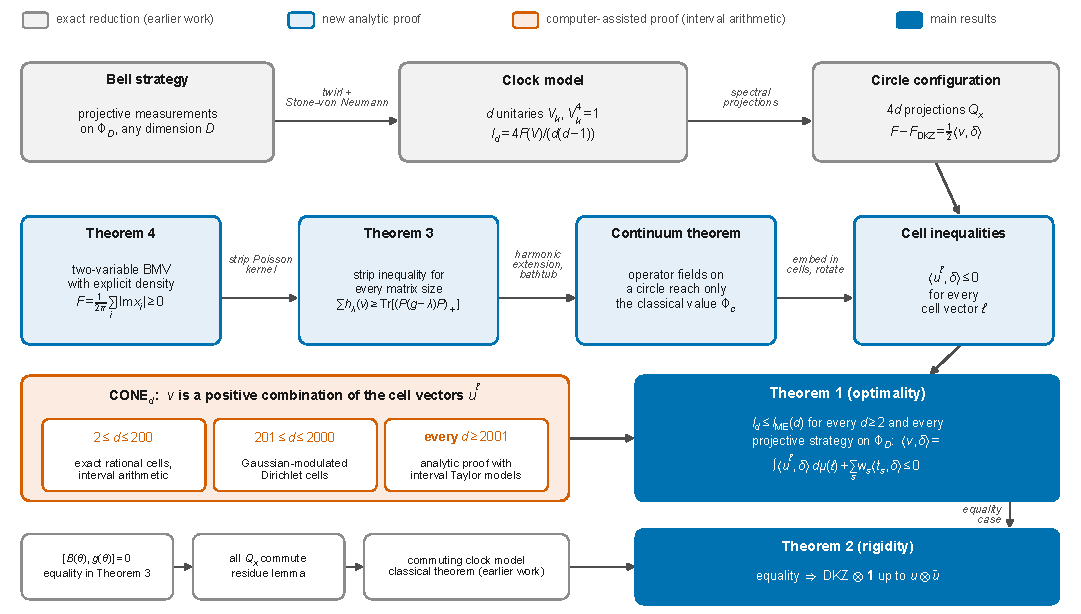
\includegraphics[width=\textwidth]{figures/fig2.pdf}
\caption{Architecture of the proof of Theorems~\ref{thm:opt} and~\ref{thm:rig}: the exact reduction
(Section~\ref{subsec:clock}), the analytic chain (Sections~\ref{subsec:strip}--\ref{subsec:cells}; the density of
Theorem~\ref{thm:bmv} is denoted $F$ in the figure and $\rho$ in the text), the certified cone condition
(Section~\ref{subsec:cone}) and the equality case (Section~\ref{subsec:proofs12}).}
\label{fig:arch}
\end{figure}

The proof has six steps (Figure~\ref{fig:arch}). (1)~An exact reduction~\cite{MSclassical} turns every strategy into a
$d$-tuple $V$ of unitaries of order four with $I_d=4F(V)/(d(d-1))$, and then into $4d$ projections on a circle, for
which $F(V)-\FD=\frac12\ip v\delta$ is a linear form in $d-1$ ``net pair counts''. (2)~Theorem~\ref{thm:bmv} implies
Theorem~\ref{thm:strip}. (3)~Through a harmonic function on the disc, Theorem~\ref{thm:strip} shows that
operator-valued fields on a circle, paired with their conjugate function, reach only the classical (commutative) value.
(4)~Placing the $4d$ projections on cells of lengths $\ell_{x\bmod d}$ and averaging over rotations gives
$\ip{u^\ell}\delta\le0$ for every cell vector, so Theorem~\ref{thm:cone} implies $\ip v\delta\le0$, which is
Theorem~\ref{thm:opt}. (5)~Theorem~\ref{thm:cone} is certified in three regimes of $d$. (6)~In the equality case every
inequality is tight; the equality clause of Theorem~\ref{thm:strip} and a residue argument force all projections to
commute, and the commutative case~\cite{MSclassical} gives Theorem~\ref{thm:rig}. The continuum problem of step~(3) is
degenerate (its maximizers include non-commuting fields~\cite[Remark~4.7]{MSmath}), and the discrete problem differs
from it by junction terms of order $d$. Step~(4) avoids estimating these terms: the cell inequalities are exact
consequences of the continuum theorem, and the discrete kernel is recovered from them by the cone condition.

\subsection{Step 1: the clock model and a linear form}\label{subsec:clock}
Put $N=4d$, $w=e^{2\pi i/d}$, $z=e^{2\pi i/N}$, and $\kappa(u)=\cot(\pi u/N)$ for $u\in\Z_N\setminus\{0\}$,
$\kappa(0)=0$. Encode a strategy on $\Phi_D$ by $U_x=\sum_aw^aP^x_a$, $U'_y=\sum_bw^bQ^y_b$ and put $R_1=U_2$,
$R_2=(U'_2)^{\mathsf T}$, $R_3=U_1$, $R_4=(U'_1)^{\mathsf T}$; every quadruple of unitaries with $R_i^d=\one$ arises in
this way, and a simultaneous conjugation $R_i\mapsto uR_iu^*$ is the local unitary $u\otimes\bar u$. For unitaries
$V_0,\dots,V_{d-1}\in U(M)$ with $V_k^4=\one$ let
\begin{equation}\label{eq:FV}
F(V)=\sum_{0\le j<k\le d-1}\Re\bigl[h_{k-j}\,\tau(V_jV_k^*)\bigr],\qquad h_m=\sec\frac{\pi m}{2d}-i\csc\frac{\pi m}{2d},
\end{equation}
and $\FD=F(\one,\dots,\one)=\sum_{m=1}^{d-1}(d-m)\sec\frac{\pi m}{2d}$. With the cyclic shift $X$ on $\C^d$ and
$W=\sum_k|k\rangle\langle k|\otimes z^kV_k$, the \emph{covariant strategy} $R^V$ on $\C^d\otimes\C^M$ is
$R^V_1=X\otimes\one$, $R^V_{i+1}=WR^V_iW^*$.

\begin{proposition}[reduction~{\cite[Theorem~2.3]{MSclassical}}]\label{prop:reduction}
$I_d(R^V)=4F(V)/(d(d-1))$ for every covariant strategy, and every projective strategy $R$ on $\Phi_D$ is unitarily
equivalent, by a simultaneous conjugation, to a direct summand of some $R^V$ ($M=4D$ suffices), with
$I_d(R)=4F(V)/(d(d-1))$. Hence Theorem~\ref{thm:opt} holds if and only if $F(V)\le\FD$ for all $M$ and all $V$ with
$V_k^4=\one$.
\end{proposition}

($V$ comes from averaging over a cyclic symmetry of order $4d$ and the Stone--von Neumann theorem for $\Z_d$; the DKZ
strategy is, up to a local unitary, $R^V$ with $M=1$, $V\equiv1$.) Commuting families were treated in~\cite{MSclassical}:

\begin{proposition}[commutative sector~{\cite[Theorem~B, Corollary~C, Proposition~2.4]{MSclassical}}]\label{prop:commutative}
If the $V_k$ commute, then $F(V)\le\FD$, with equality if and only if every joint eigenvector $v$ satisfies
$V_kv=i^{-a_k}v$ with $a_k=c+[k\ge r]$ for some $c\in\Z_4$, $0\le r\le d-1$. A strategy has commuting reduced family if
and only if its four link operators coincide, $R_1^nR_2^{-n}=R_2^nR_3^{-n}=R_3^nR_4^{-n}=w^{-n}R_4^nR_1^{-n}$ for all
$n$; and if such a strategy attains $\IME(d)$, then $d\mid D$ and $uR_iu^*=R_i^{\DKZ}\otimes\one$ for a unitary $u$.
\end{proposition}

A \emph{Q-configuration} on $\C^M$ is a family $(Q_x)_{x\in\Z_N}$ of projections such that for each
$k\in\{0,\dots,d-1\}$ the four projections $Q_{k-da}$, $a\in\Z_4$, are pairwise orthogonal with sum $\one$; put
$A_x=Q_x$, $B_x=Q_{x+d}$ and $(\mathrm{rot}_jQ)_x=Q_{x-j}$. Taking for $Q_{k-da}$ the spectral projection of $V_k^*$ for
the eigenvalue $i^a$ is a bijection between families $V$ and Q-configurations; $V\equiv\one$ gives the \emph{window}
$Q_x=\one_{[0,d)}(x)$. Since each residue class modulo $d$ carries a projective measurement,
$\sum_x\ell_xA_x=\sum_x\ell_xB_x=(\sum_{r<d}\ell_r)\one$ for every $d$-periodic $\ell$.

\begin{lemma}[linear form~{\cite[eq.~(13)]{MSclassical}, \cite[Lemmas~2.4, 2.5]{MSmath}}]\label{lem:linearform}
Let $T(m)=\sum_y\tau(A_{y+m}B_y)$, $\cN(m)=T(m)-T(-m)$ and $\delta_m=\cN(m)-m$ for $1\le m\le d-1$. Then
$F(V)=\frac12\sum_{x,y}\kappa(x-y)\tau(A_xB_y)-\frac d2$, the window has $\cN(m)=m$, and
\[
F(V)-\FD=\tfrac12\ip v\delta,\qquad \ip{t_s}\delta=\cN(s)+\cN(d-s)-d\le0\quad(1\le s\le d-1).
\]
\end{lemma}

(The first formula follows from $\sec t=\frac12[\cot(\frac t2+\frac\pi4)-\cot(\frac t2-\frac\pi4)]$, the second from
$\cN(2d-m)=\cN(m)$, $\cN(d)=d$ and $\cot\frac{\pi m}{4d}+\tan\frac{\pi m}{4d}=2\csc\frac{\pi m}{2d}$, and the last because
$\cN(s)+\cN(d-s)$ is a sum of $d$ differences of probabilities, each at most $1$.) So Theorem~\ref{thm:opt} is
equivalent to
\begin{equation}\label{eq:target}
\ip v\delta\le0\qquad\text{for every Q-configuration on every }\C^M .
\end{equation}

\subsection{Step 2: the strip inequality from an explicit positive density}\label{subsec:strip}
Let $g_{\mathrm d}=BgB+PgP$, $K=[\lmin,\lmax]\times[0,1]$, and for $s\in\R$, $0<\tau<1$ let
$p_{s,\tau}(\xi)=\det(g-s-\xi(P-\tau))$ and $q_{s,\tau}(\xi)=\det(g_{\mathrm d}-s-\xi(P-\tau))$. The roots of
$p_{s,\tau}$ are the eigenvalues of $(P-\tau)^{-1}(g-s)$, which is self-adjoint for an indefinite inner product.

\begin{lemma}[pencil facts~{\cite[Lemmas~3.3, 3.4]{MSmath}}]\label{lem:pencil}
\textup{(1)} $p_{s,\tau}$ and $q_{s,\tau}$ have degree $M$, the same leading coefficient and the same sum of roots;
all roots of $q_{s,\tau}$ are real; every non-real root $\xi$ of $p_{s,\tau}$ satisfies
$|\xi|\le\|g-s\|/\sqrt{\tau(1-\tau)}$; and all roots of $p_{s,\tau}$ are real if $s\notin(\lmin,\lmax)$.
\textup{(2)} If $p(\xi)=c\prod_i(\xi-\xi_i)$ and $q(\xi)=c\prod_i(\xi-y_i)$ with $c\ne0$, all $y_i$ real and
$\sum_i\xi_i=\sum_iy_i$, then $\int_\R\log|p(\xi)/q(\xi)|\dd\xi=\pi\sum_i|\Im\xi_i|$.
\end{lemma}

\begin{proof}[Outline of the proof of Theorem~\ref{thm:bmv} \textup{(\cite[Section~3.5]{MSmath})}]
$\cD/a^2$ is entire on $\C^2$ and grows at most like the exponential of
$\max_{(s,\tau)\in K}(s\Re a-\tau\Re t)$, so by the Paley--Wiener--Schwartz theorem~\cite[Theorem~7.3.1]{Hormander} it is
the Laplace transform of a distribution $\Theta$ supported in $K$. On the line $t=a\xi$ it is the Laplace transform of
\[
U_\xi(w)=\sum_j\bigl[(w-\lambda_j(\xi))_+-(w-\lambda^0_j(\xi))_+\bigr],
\]
where $\lambda_j(\xi)$ and $\lambda^0_j(\xi)$ are the eigenvalues of $g-\xi P$ and $g_{\mathrm d}-\xi P$; the Hilbert
transform of $U_\xi'$ is $\frac1\pi\log|\det(g-\xi P-w)/\det(g_{\mathrm d}-\xi P-w)|$, which at $w=s-\xi\tau$ equals
$\frac1\pi\log|p_{s,\tau}(\xi)/q_{s,\tau}(\xi)|$. Fourier inversion one line at a time and Lemma~\ref{lem:pencil}(2) give
$\Theta=\rho$ on $\R\times(0,1)$; the limits of $\Tr e^{ag-tP}$ as $t\to\pm\infty$ exclude mass on the edges
$\tau\in\{0,1\}$; and Duhamel's formula, $\frac12\partial_a^2\cD(0,t)=\|BgP\|_F^2(1-e^{-t})/t$, gives the marginal
identity.
\end{proof}

A second proof avoids distributions, Paley--Wiener theory and Fourier inversion in two variables; it is the route
formalised in Lean.

\begin{proposition}[Radon identity~{\cite[Theorem~B.1]{MSmath}}]\label{prop:radon}
For Hermitian $H$ let $y_1(\tau),\dots,y_M(\tau)$ be the eigenvalues of $(P-\tau)^{-1}H$, $0<\tau<1$. Then
$\sum_i|\Im y_i(\tau)|\le M\|H\|/\sqrt{\tau(1-\tau)}$ is continuous in $\tau$, and
$\frac1{2\pi}\int_0^1\sum_i|\Im y_i(\tau)|\dd\tau=\Tr H_+-\Tr(BHB+PHP)_+$.
\end{proposition}

\begin{proof}[Outline]
For $H+c$ with $\Im c>0$ no root is real and exactly $\operatorname{rank}P$ roots lie in the upper half-plane $\C_+$. The
roots obey the complex inviscid Burgers equation $\partial_\tau y=y\,\partial_cy$; summed over the roots in $\C_+$
through a Cauchy integral, valid also at multiple roots, it gives
$\partial_\tau\sum_{\C_+}\operatorname{Log}y=\partial_c\sum_{\C_+}y$. Integrating over $\tau$ and evaluating the two ends
by a Schur complement identifies $\int_0^1\sum_{\C_+}y\,\dd\tau$, minus the same quantity for $H_{\mathrm d}=BHB+PHP$,
with $\Tr[(H_{\mathrm d}+c)\operatorname{Log}(H_{\mathrm d}+c)]-\Tr[(H+c)\operatorname{Log}(H+c)]$ up to an affine
function of $c$, which vanishes (consider $c>\|H\|$). Imaginary parts as $c$ tends to the real axis give the identity.
\end{proof}

Applied to $H=g-\xi P-w$, Proposition~\ref{prop:radon} says that the integrals of $\rho$ along the lines $s=w+\xi\tau$
are the functions $U_\xi(w)$; Tonelli's theorem for real $(a,t)$ and the identity theorem then give~\eqref{eq:bmv} on
$\C^2$~\cite[Section~B.4]{MSmath}. The same argument with an arbitrary Hermitian matrix in place of $P$ gives a proof
of Stahl's theorem without distribution theory or Fourier analysis; we make no priority claim about this
by-product~\cite[Remark~B.8]{MSmath}.

\begin{proof}[Outline of the proof of Theorem~\ref{thm:strip} \textup{(\cite[Section~3.6]{MSmath})}]
The eigenvalues $\nu_k=x_k+iy_k$ of $B+ig$ have $x_k\in[0,1]$, because $\Re\ip v{(B+ig)v}=\ip v{Bv}$. Let $\omega$ be
the sum of the harmonic measures of $S$ at the $\nu_k$ restricted to the left edge (the measures $K_{x_k}(y_k-w)\dd w$),
and $\sigma$ the eigenvalue counting measure of $PgP$ on $\operatorname{ran}P$; the left side of~\eqref{eq:strip} is
$\int(w-\lambda)_+\dd(\omega-\sigma)$. For real $0<|a|<\pi$ the Laplace transform of $\omega$ is
$[\Tr e^{ag+iaP}-\Tr e^{ag-iaP}]/(2i\sin a)$ and that of $\sigma$ is $\Tr_Pe^{aPgP}$; by~\eqref{eq:bmv} at $t=\mp ia$
and $\int e^{-au}K_{1-\tau}(u)\dd u=\sin(a\tau)/\sin a$, their difference is the Laplace transform of $a^2V$,
$V(w)=\iint K_{1-\tau}(s-w)\rho(s,\tau)\dd s\dd\tau$. So $\omega-\sigma$ has zero mass and first moment, and
$W(w)=\int(w-u)_+\dd(\omega-\sigma)(u)$ has the same Laplace transform as $V$; both are continuous and
$O(e^{-\pi|w|})$, so $W=V$, which at $w=\lambda$ is~\eqref{eq:strip}. If the defect vanishes for one $\lambda$, then
$\rho\equiv0$, so $\cD\equiv0$ and $\|BgP\|_F=0$, that is, $[B,g]=0$.
\end{proof}

Equivalently, Theorem~\ref{thm:strip} says that $\sigma$ is dominated by $\omega$ in the convex order, a Schur--Horn
type majorization for the non-normal matrix $B+ig$. For $\operatorname{rank}B\le1$ there is a second proof, by an
argument-principle count, which also covers $\operatorname{rank}P\le3$ and hence all $M\le5$~\cite[Remark~3.10]{MSmath}.

\subsection{Step 3: a noncommutative continuum theorem}\label{subsec:continuum}
Let $\T=\R/2\pi\Z$ with $\dd m=\dd\theta/2\pi$. A \emph{projection step field} is a function $B(\theta)=B_j$ on arcs
$(t_j,t_{j+1})$, $t_0<\dots<t_{n-1}<t_0+2\pi$, with projections $B_j$ on $\C^M$. Its conjugate function
$g(\theta)=\mathrm{p.v.}\!\int_\T\cot\frac{\theta-\varphi}2B(\varphi)\dd m(\varphi)=\frac1\pi\sum_j(B_j-B_{j-1})\log|\sin\frac{\theta-t_j}2|$
is Hermitian and real-analytic on each arc. For $\alpha,\beta\ge0$ with $\alpha+\beta\le1$ let
$\Phic(\alpha,\beta)=\frac1{2\pi^2}[\Cl(2\pi\alpha)+\Cl(2\pi\beta)+\Cl(2\pi(1-\alpha-\beta))]$, so that
$\Phic(\frac14,\frac14)=G/\pi^2$.

\begin{proposition}[continuum theorem~{\cite[Theorem~4.2]{MSmath}}]\label{prop:continuum}
Let $B$ be a projection step field on $\C^M$ with conjugate function $g$, $P=\one-B$, and $A$ a measurable field with
$0\le A\le P$. Put $\alpha=\int\tau(A)\dd m$, $\beta=\int\tau(B)\dd m$, and let $\beta_1,\dots,\beta_M$ be the
eigenvalues of $\int B\dd m$. For every $\lambda\in\R$,
\[
\lambda\alpha+h_\lambda(\beta)-\int_\T\tau(Ag)\dd m=\Bigl[h_\lambda(\beta)-\frac1M\sum_ih_\lambda(\beta_i)\Bigr]
+\frac1M\int_\T D_\lambda\dd m+\int_\T S_\lambda\dd m ,
\]
where $D_\lambda(\theta)\ge0$ is the left side of~\eqref{eq:strip} for the pair $(B(\theta),g(\theta))$,
$S_\lambda=\tau[(P(g-\lambda)P)_+]-\tau[A(g-\lambda)]\ge0$, and the bracket is nonnegative. Moreover
$\min_\lambda[\lambda\alpha+h_\lambda(\beta)]=\Phic(\alpha,\beta)$ for $\alpha,\beta>0$, $\alpha+\beta<1$; at
$\alpha=\beta=\frac14$ the minimum $G/\pi^2$ is attained only at $\lambda^*=\frac{\log2}{2\pi}$.
\end{proposition}

\begin{proof}[Outline]
$D_\lambda\ge0$ is Theorem~\ref{thm:strip}, $S_\lambda\ge0$ is a bathtub argument, and the bracket is nonnegative by
concavity of $x\mapsto h_\lambda(x)$ on $[0,1]$. The Herglotz function $\mathcal F(z)=\int\frac{e^{i\varphi}+z}{e^{i\varphi}-z}B(\varphi)\dd m(\varphi)$
is holomorphic on the disc with $\mathcal F(0)=\int B\dd m$ and boundary values $B+ig$, and its spectrum lies in the closed
strip. As $h_\lambda=\Re\phi_\lambda$ with $\phi_\lambda(z)=\frac i{\pi^2}\Li(e^{-i\pi z-\pi\lambda})$ holomorphic on $S$,
$z\mapsto\sum_{\nu\in\spec\mathcal F(z)}h_\lambda(\nu)$ is harmonic, and its boundary mean equals its value at the
centre. The minimum is a Legendre-type identity for the dilogarithm~\cite[Lemma~4.4]{MSmath}.
\end{proof}

\begin{corollary}[equality~{\cite[Corollary~4.5]{MSmath}}]\label{cor:equality}
If $\int B\dd m=\frac14\one$ and $\int\tau(A)\dd m=\frac14$, then $\frac G{\pi^2}-\int\tau(Ag)\dd m=\frac1M\int
D_{\lambda^*}\dd m+\int S_{\lambda^*}\dd m\ge0$; if equality holds, $[B(\theta),g(\theta)]=0$ for almost every $\theta$.
\end{corollary}

\subsection{Step 4: cell embeddings}\label{subsec:cells}
For $\ell\in\Delta_d$, extended by $\ell_x=\ell_{x\bmod d}$, put $L_0=0$, $L_{x+1}=L_x+\ell_x$ and
$I_x=[L_x,L_{x+1})\subseteq\R/N\Z$, so that $S_r(m)=L_{r+m}-L_r$. For $x\ne y$ let
$K^\ell(x,y)=\int_{I_x}\int_{I_y}\cot\frac{\pi(\xi-\eta)}N\dd\eta\dd\xi$, which equals
$\Xi(L_{x+1}-L_y)-\Xi(L_x-L_y)-\Xi(L_{x+1}-L_{y+1})+\Xi(L_x-L_{y+1})$ since $\Xi''(u)=\cot\frac{\pi u}N$; let
$K^\ell(x,x)=0$ and $Q^\ell(Q)=\sum_{x,y}K^\ell(x,y)\tau(A_xB_y)$.

\begin{proposition}[cell inequalities~{\cite[Propositions~5.2, 5.3]{MSmath}}]\label{prop:average}
For every $\ell\in\Delta_d$ and every Q-configuration, $Q^\ell(Q)\le N^2G/\pi^2$, with equality for every window, and
$\frac1d\sum_{j=0}^{d-1}[Q^\ell(\mathrm{rot}_jQ)-N^2G/\pi^2]=\ip{u^\ell}\delta$; hence $\ip{u^\ell}\delta\le0$.
\end{proposition}

\begin{proof}[Sketch]
Let $B$ and $A$ be the step fields on $\T$ equal to $B_x$ and $A_x$ on the arc $(2\pi L_x/N,2\pi L_{x+1}/N)$. Then
$0\le A\le\one-B$, $\int B\dd m=\int A\dd m=\frac1N\sum_x\ell_xB_x=\frac14\one$, and $Q^\ell(Q)=N^2\int\tau(Ag)\dd m$, so
Corollary~\ref{cor:equality} applies; for a window, $A$ and $B$ are indicators of two adjacent arcs of length $d$, with
value $N^2\Phic(\frac14,\frac14)$. The rotation average depends only on $x-y$, and subtracting the window value gives
$\ip{u^\ell}\delta$, with $u^\ell$ as in~\eqref{eq:uell}.
\end{proof}

\begin{proposition}[the cone condition implies optimality]\label{prop:conetoopt}
If $v=\int u^\ell\mu(\dd\ell)+\sum_sw_st_s$ with $\mu\ge0$ and $w_s\ge0$, then $\ip v\delta\le0$ for every
Q-configuration. Hence Theorem~\ref{thm:cone} implies Theorem~\ref{thm:opt}.
\end{proposition}

\begin{proof}
$\ip v\delta=\int\ip{u^\ell}\delta\mu(\dd\ell)+\sum_sw_s\ip{t_s}\delta\le0$ by Proposition~\ref{prop:average} and
Lemma~\ref{lem:linearform} ($\ell\mapsto u^\ell$ is continuous on the compact set $\Delta_d$); conclude
with~\eqref{eq:target}.
\end{proof}

For uniform cells, $u^1=v+j$ with $j_m\ge0$ made of junction terms, so non-uniform cells are needed. Cells with
$\ell/d$ uniform on the simplex give $\E u^\ell_m=\int_0^d(\Sh)''(s)b_{m,d}(s/d)\dd s$ ($b_{m,d}$ a Bernstein polynomial),
which reproduces exactly the singular part $\frac{4d}{\pi m}$ of $v_m$ and leaves a smooth residual of relative size
$O(1/d)$, corrected in Section~\ref{subsec:cone}.

\subsection{Step 5: the cone condition for every \texorpdfstring{$d$}{d}}\label{subsec:cone}
This step is computer-assisted, in interval arithmetic with outward rounding (\texttt{mpmath}~\cite{mpmath}; 160 bits
for $d\le2000$, $120$--$240$ bits beyond). For a probability measure $\mu$ on $\Delta_d$ let
$P_\mu(m)=\int\frac1d\sum_r\Sh(S_r(m))\mu(\dd\ell)$ ($0\le m\le d$), so that $\int u^\ell\dd\mu=\Delta^2P_\mu$, and let $P_v$
solve $\Delta^2P_v=v$ with the same boundary values $\Sh(0)$, $\Sh(d)$.

\begin{lemma}[reduction to potentials]\label{lem:potentials}
If \textup{(i)} the antisymmetric parts of $P_\mu$ and $P_v$ under $m\mapsto d-m$ agree, and \textup{(ii)} the symmetric
part $W$ of $P_v-P_\mu$ satisfies $\Delta^2W\ge0$ on $\{1,\dots,d-1\}$, then~\eqref{eq:cone} holds with this $\mu$.
\end{lemma}

\begin{proof}
$W(0)=W(d)=0$ and $P_\mu+W=P_v$, so $\int u^\ell\dd\mu+\Delta^2W=v$, and $\Delta^2W$ is symmetric and nonnegative,
hence a nonnegative combination of the $t_s$.
\end{proof}

\paragraph{Regime I: $2\le d\le200$ \textup{(\cite[Proposition~6.2]{MSmath})}.}
Here $\mu=\sum_kc_k\delta_{\ell^{(k)}}$ and $w=0$, with $K_d\le6.3\,d$ cell vectors $\ell^{(k)}=n^{(k)}/16$ (integers
$n^{(k)}_r\ge1$) and certified weights $c_k>0$, $d\cdot\min_kc_k\ge0.0816$. The Clausen values are enclosed by the
Bernoulli series with exact Bernoulli numbers and an explicit tail bound. Weights found by floating-point linear
programming (HiGHS~\cite{HiGHS}, not part of the verification) are corrected to an exact solution of
$\sum_kc_ku^{\ell^{(k)}}=v$ through a certified residual bound ($\|\one-RUU^{\mathsf T}\|_\infty\le9.4\cdot10^{-34}$
for an approximate inverse $R$ of $UU^{\mathsf T}$, $U$ the matrix of the $u^{\ell^{(k)}}$). The smallest weight is
$4.25\cdot10^{-4}$ ($d=198$); all $199$ certificates were re-verified, and for $d\le20$ they are also evaluated by the
Lean kernel in exact rational arithmetic.

\paragraph{Regimes II and III: $d\ge201$.}
Here $\mu$ is the law of a random cell vector: $d$ times a Dirichlet vector with parameters $1+\eta_r$, where
$\eta$ is a stationary centred Gaussian vector on $\Z_d$ with $\sum_r\eta_r=0$, conditioned on $\max_r|\eta_r|<\frac34$
(parameters $1$ otherwise). The unknown is the variogram $\Upsilon(m)=\operatorname{Var}(\eta_r+\dots+\eta_{r+m-1})$,
which must have positive cosine coefficients $\hat a_k(\Upsilon)$ to define a covariance. By Dirichlet aggregation,
$P_\mu$ becomes an average of Beta expectations of $\Sh$, which reproduce the singular part of $P_v$ exactly (a digamma
identity~\cite[Lemma~6.3]{MSmath}). Condition~(i) of Lemma~\ref{lem:potentials} then decouples, up to an error
$O(d^3\log d\,e^{-9/(32\Upsilon(1))})$, into one scalar equation per distance $m<d/2$, and a Poincar\'e--Miranda
argument~\cite{Kulpa} on a box of variograms passes from the decoupled to the exact equations~\cite[Lemmas~6.4,
6.5]{MSmath}. It remains to certify, on the whole box, the positivity of the $\hat a_k$, the sign conditions on the
faces, and condition~(ii).

For $201\le d\le2000$ \textup{(\cite[Proposition~6.6]{MSmath})}, one run per $d$ of \texttt{verify\_cert.py} (one
process, $160$-bit arithmetic, one code version whose SHA-256 hash is stored in every certificate) encloses the
decoupled solution (an exact Gaussian expansion of order $14$ with an order-$16$ remainder) and certifies all conditions
on the whole box, with exact factorials, binomial coefficients and Bernoulli numbers, rigorous Euler--Maclaurin
enclosures of $\zeta$-values, and every decision a comparison of interval endpoints; \texttt{audit\_cert\_g.py} re-checks
all $1800$ certificates from the stored exact values (all pass). The smallest margins are $d^2\min_k\hat a_k\ge0.06319$
(even $d$) and $\ge0.12638$ (odd $d$), $d\cdot\min\Delta^2W\ge0.660$, a derivative bound $4.0009$ times the required
value, and a decoupling error at most $2\cdot10^{-31.16}$.

For $d\ge2001$ \textup{(\cite[Proposition~6.8 and Appendix~A]{MSmath})}, the construction is treated uniformly in $d$,
with $\varepsilon=1/d$. An explicit real-analytic model $\Upsilon_e$ (the root of a quartic equation with special-function
coefficients) approximates the decoupled solution to within $6.6468\cdot10^{-4}\varepsilon^2$. A Fej\'er--P\'olya argument
reduces the positivity of the $\hat a_k$ to lower bounds on fourth differences of $\Upsilon_e$ minus an explicit
correction, which are certified by interval Taylor models on boxes in $(m/d,\varepsilon)$ with
$\varepsilon\in[0,1/2001]$, each box covering all $d\ge2001$ at once (at least $7.419$ in the outer zone
$0.011\le m/d\le0.501$, at least $6.022431$ in the inner zone, and directly for $m=1,2$). The result is
$\hat a_k\ge w_k(0.1186944\,\varepsilon^2-2\varrho)>0$ ($w_k\in\{\frac12,1\}$, $\varrho\le e^{-837}$ the box radius),
second differences of the symmetric slack at least $0.620154\,\varepsilon-4\varrho d^2$, and logarithmic margins above
$800$ for the tail and fixed-point conditions. A final rigour pass fixed code-level enclosure defects (one had left a
sliver of size about $10^{-20}$ uncovered at $d=2001$); no conclusion changed.

In all regimes $\mu$ is carried by $\Delta_d^+$ (all cells $\ge\frac1{16}$ in Regime~I; Dirichlet parameters $\ge\frac14$
beyond), as Theorem~\ref{thm:cone} requires. The single command \texttt{python audit\_alld.py} re-checks all three regimes
and prints \texttt{ALL-D CERTIFIED (every d >= 2)}. In Lean, $\CONE_d$ is used in a finite form (finitely many cell
vectors, one with all cells positive); for $d\ge201$ it follows from the integral form by Carath\'eodory's theorem, each
$t_s$ being a positive multiple of a cell vector supported on two residues~\cite[Remark~11.1]{MSmath}.

\subsection{Step 6: proofs of Theorems~\ref{thm:opt} and~\ref{thm:rig}}\label{subsec:proofs12}
Theorem~\ref{thm:opt} follows from Theorem~\ref{thm:cone} and Proposition~\ref{prop:conetoopt}; the DKZ strategy attains
$\IME(d)$ by Proposition~\ref{prop:reduction}.

\begin{proposition}[pointwise commutation forces commutation~{\cite[Lemma~7.2, Proposition~7.3]{MSmath}}]\label{prop:residue}
Let $\ell\in\Delta_d^+$, let $Q$ be a Q-configuration, and let $B$, $g$ be the step field and conjugate function of the
proof of Proposition~\ref{prop:average}. If $[B(\theta),g(\theta)]=0$ for almost every $\theta$, then all $Q_x$ commute.
\end{proposition}

\begin{proof}
All cells are nonempty, so the endpoints $t_x=2\pi L_x/N$ are distinct modulo $2\pi$. On the arc of $x$, $B=B_x$ and $g$
is real-analytic, so $[B_x,g(\theta)]$ and its derivative $\frac1{2\pi}\sum_j[B_x,B_j-B_{j-1}]\cot\frac{\theta-t_j}2$
vanish identically there. This meromorphic function of $\theta$ then vanishes everywhere, and its residue at $t_j$ is
$\frac1\pi[B_x,B_j-B_{j-1}]$; so $j\mapsto[B_x,B_j]$ is constant, equal to $[B_x,B_x]=0$. The $B_x=Q_{x+d}$ run over all
the $Q$'s.
\end{proof}

\begin{proof}[Proof of Theorem~\ref{thm:rig}]
Let a strategy attain $\IME(d)$; then $\ip v\delta=0$ for its Q-configuration. By Theorem~\ref{thm:cone},
$0=\int\ip{u^\ell}\delta\mu(\dd\ell)+\sum_sw_s\ip{t_s}\delta$ with nonpositive terms, so the continuous function
$\ell\mapsto\ip{u^\ell}\delta$ vanishes $\mu$-almost everywhere, and as $\mu(\Delta_d^+)>0$ some $\ell^*\in\Delta_d^+$ has
$\ip{u^{\ell^*}}\delta=0$. By Proposition~\ref{prop:average} the $d$ nonpositive numbers
$Q^{\ell^*}(\mathrm{rot}_jQ)-N^2G/\pi^2$ have mean $0$, so $Q^{\ell^*}(Q)=N^2G/\pi^2$; Corollary~\ref{cor:equality} gives
$[B(\theta),g(\theta)]=0$ almost everywhere, and Proposition~\ref{prop:residue} that all $Q_x$, hence all $V_k$, commute.
Proposition~\ref{prop:commutative} gives $d\mid D$ and $uR_iu^*=R_i^{\DKZ}\otimes\one$; spectral projections and
transposition give the statements about $P^x_a$ and $Q^y_b$, and $(u\otimes\bar u)\sum_i|ii\rangle=\sum_j|jj\rangle$ for
every unitary $u$. If $u_1,u_2$ both work, $u_2u_1^*$ commutes with the $R_i^{\DKZ}\otimes\one$, which generate
$M_d(\C)\otimes\one$, so $u_2u_1^*\in\one_d\otimes U(D/d)$. Finally, for fixed $D$ the maximum of $I_d$ is attained (by
compactness), so it equals $\IME(d)$ only if $d\mid D$.
\end{proof}

\begin{remark}[a deficit identity, and $d\to\infty$]\label{rem:limit}
The proof writes the deficit $\FD-F(V)$ of every strategy as an explicit positive combination of integrated defects of
Theorem~\ref{thm:strip}, bathtub slacks and pair slacks~\cite[Remark~7.1]{MSmath}, which suggests a quantitative form of
Theorem~\ref{thm:rig}. As $d\to\infty$, $\IME(d)=32G/\pi^2-c_1/d+O(d^{-2})$ with
$c_1=2+\frac4\pi-\frac{32G}{\pi^2}=0.30342\ldots$~\cite[Corollary~8.1]{MSmath}.
\end{remark}

\subsection{General measurements for \texorpdfstring{$3\le d\le8$}{3 <= d <= 8}}\label{subsec:povm}
The reduction of Section~\ref{subsec:clock} uses projections in an essential way, and the exact certificates
of~\cite{repoCGLMP} for $d\le20$ use the group law $R_i^nR_i^m=R_i^{n+m}$, $R_i^d=\one$, so neither covers POVMs. For small $d$ a
separate certificate does.

\begin{proposition}[POVMs; computer-assisted]\label{prop:povm}
Let $3\le d\le8$ and $D\ge1$. For all $d$-outcome POVMs, two for each party, on $\Phi_D$, $I_d\le\IME(d)$; and equality
forces all four POVMs to be projective, so that Theorem~\ref{thm:rig} applies.
\end{proposition}

\begin{proof}[Sketch]
With $E^0,E^2$ Alice's POVMs, $E^1,E^3$ the transposes of Bob's, and $Z^g_n=\sum_aw^{na}E^g_a$, the CGLMP deficit (up to
a relabelling of settings and a positive factor) is the normalised trace of an element $S_{\mathrm{op}}-\lambda_d$ of the free $*$-algebra of the
effects, in which only $Z^g_0=\one$ and $(Z^g_n)^*=Z^g_{-n}$ are used (no idempotence). After symmetrisation over a group
of order $16d$, an exact identity over $\mathbb Q(e^{2\pi i/4d})$ writes it, modulo cyclic rotation and the symmetry
relations, as a sum of Hermitian squares of combinations of the words $1$, $Z^g_n$, $Z^g_nZ^{g\pm1}_m$ (level ``1+AB''
of the tracial moment relaxation) and doubly-localizing terms $\tau(f^*EfF)\ge0$ ($E$ an effect of Alice, $F$ one of
Bob), with Gram blocks proved positive definite by exact $LDL^{\mathsf T}$ factorisation and by interval Cholesky
factorisation. In the equality case the kernels of the certificate force $E^0_cZ^0_nE^1_b=w^{nc}E^0_cE^1_b$ and
$E^0_cZ^1_nE^1_b=w^{nb}E^0_cE^1_b$, so the POVMs are projective.
\end{proof}

%==============================================================================================================
\section{Clause 27B(ii): resistance to noise}\label{sec:noise}
%==============================================================================================================

\subsection{Three readings}\label{subsec:readings}
In Gill's paper~\cite{Gill} the noise is the behaviour $p_0$ of uniformly random outcomes, and the resistance of a
violation is measured by how much of $p_0$ can be admixed while local realism is still violated, that is, by the
critical visibility $\vc$. For strategies on maximally entangled states the clause can be read in three ways:
(a)~\emph{CGLMP reading}: noise $p_0$, nonlocality detected by the CGLMP inequality $I_d\le2$;
(b)~\emph{Gill's literal reading}: noise $p_0$, nonlocality against all Bell inequalities, that is, $\vc$;
(c)~\emph{white-noise reading} (a strengthening): noise on the state, $v|\Phi_D\rangle\langle\Phi_D|+(1-v)\one/D^2$, and
nonlocality against all Bell inequalities. In~(c) the noise contributes the product behaviour $\Tr P^x_a\,\Tr
Q^y_b/D^2$, which equals $p_0$ if every outcome of every measurement has trace $D/d$, for example for rank-one
measurements on $\Phi_d$. Reading~(a) holds for every $d$ (Theorem~\ref{thm:noisecglmp}), reading~(b) fails for every
$d\ge4$ (Theorem~\ref{thm:literal}), and reading~(c) is open for $d\ge4$ (Section~\ref{subsec:white}).

\subsection{The CGLMP reading}\label{subsec:noisecglmp}

\begin{theorem}[noise resistance of the CGLMP violation]\label{thm:noisecglmp}
Let $d\ge2$, $D\ge1$, let $p$ be the behaviour of a projective strategy $\mathcal S$ on $\Phi_D$, and
$p_v=vp+(1-v)p_0$. \textup{(1)} $I_d(p_v)=vI_d(p)$; hence $p_v$ violates $I_d\le2$ if and only if $vI_d(p)>2$.
\textup{(2)} The CGLMP noise threshold $v_{\mathrm{CGLMP}}(\mathcal S)=\inf\{v\in[0,1]:I_d(p_v)>2\}$ equals $2/I_d(p)$
if $I_d(p)>2$ \textup{(}and $+\infty$ otherwise\textup{)}, and $v_{\mathrm{CGLMP}}(\mathcal S)\ge2/\IME(d)$.
\textup{(3)} $v_{\mathrm{CGLMP}}(\DKZ_d)=2/\IME(d)$, and $v_{\mathrm{CGLMP}}(\mathcal S)=2/\IME(d)$ if and only if $d\mid
D$ and $\mathcal S$ is $\DKZ_d\otimes\one_{D/d}$ up to a local unitary $u\otimes\bar u$. The same holds for white noise
on the state whenever every outcome of every measurement has trace $D/d$.
\end{theorem}

\begin{proof}
(1) $I_d$ is linear and $I_d(p_0)=0$. (2) If $I_d(p)>2$, the violating $v\in[0,1]$ form $(2/I_d(p),1]$, and
$I_d(p)\le\IME(d)$ by Theorem~\ref{thm:opt}. (3) $I_d(p_{\DKZ})=\IME(d)$; conversely
$v_{\mathrm{CGLMP}}(\mathcal S)=2/\IME(d)$ forces $I_d(p)=\IME(d)$, and Theorem~\ref{thm:rig} applies, while the behaviour
is invariant under $u\otimes\bar u$ and inert identities. Under the trace condition the maximally mixed state gives
$\Tr(P^x_a)\Tr(Q^y_b)/D^2=d^{-2}$.
\end{proof}

Theorem~\ref{thm:noisecglmp} is formalised in Lean (file \texttt{CglmpNoise.lean}; Table~\ref{tab:lean}): for every
behaviour, mixing with uniform noise multiplies the CGLMP value by $v$ (\nolinkurl{OQP27.cglmpOf_noisy}); parts~(2)
and~(3) hold for $2\le d\le20$ with no hypothesis and for every $d$ given $\CONE_d$ for $d\ge21$. It concerns the CGLMP
inequality only. For outcomes of unequal traces, white noise on the state produces a local behaviour whose CGLMP value
need not vanish, and the theorem says nothing about it (Section~\ref{sec:open}). For $3\le d\le8$,
Proposition~\ref{prop:povm} extends Theorem~\ref{thm:noisecglmp} to POVMs. For all Bell inequalities the corresponding
statement is false for every $d\ge4$, as we show next.

\subsection{Gill's literal reading}\label{subsec:literal}
Let $\sA_1=\sigma_z$, $\sA_2=\sigma_x$, $\sB_1=(\sigma_z+\sigma_x)/\sqrt2$ and $\sB_2=(\sigma_z-\sigma_x)/\sqrt2$ be the
optimal CHSH observables, and $\Pi^x_\pm=\frac12(\one\pm\sA_x)$, $\Pi'^y_\pm=\frac12(\one\pm\sB_y)$, real symmetric
rank-one projections on $\C^2$. For $d\ge3$ define a projective strategy $C_d$ on $\Phi_d$ as follows. For even $d$,
identify $\C^d=\C^2\otimes\C^{d/2}$ by $|i\rangle|j\rangle\mapsto|i\frac d2+j\rangle$, so that $\Phi_d=\Phi_2\otimes\Phi_{d/2}$,
and let $P^x_0=\Pi^x_+\otimes\one$, $P^x_1=\Pi^x_-\otimes\one$, $Q^y_0=\Pi'^y_+\otimes\one$, $Q^y_1=\Pi'^y_-\otimes\one$.
For odd $d$, decompose $\C^d=\bigoplus_{k=1}^{(d-1)/2}\operatorname{span}\{|2k-2\rangle,|2k-1\rangle\}\oplus\C|d-1\rangle$
and let $P^x_0=(\bigoplus_k\Pi^x_+)\oplus1$, $P^x_1=(\bigoplus_k\Pi^x_-)\oplus0$, and $Q^y_0,Q^y_1$ likewise with
$\Pi'^y_\pm$. In both cases $P^x_a=Q^y_b=0$ for $a,b\ge2$: the outcomes $2,\dots,d-1$ never occur. Put
\begin{equation}\label{eq:vevenodd}
\veven(d)=\frac{4(d-1)}{(\sqrt2-1)d^2+4(d-1)},\qquad\vodd(d)=\frac4{(\sqrt2-1)d+4}.
\end{equation}

\begin{theorem}[Gill's noise clause; computer-assisted for $4\le d\le9$]\label{thm:literal}
\textup{(1)} For every $d\ge3$, $\vc(C_d)=\veven(d)$ if $d$ is even and $\vc(C_d)=\vodd(d)$ if $d$ is odd.
\textup{(2)} For every $d\ge2$, $\frac12\le\vc(\DKZ_d)\le2/\IME(d)$; for $4\le d\le9$, $\vc(\DKZ_d)\ge r(d)$, where
$r(4),\dots,r(9)=0.69,\ 0.687,\ 0.684,\ 0.683,\ 0.682,\ 0.681$.
\textup{(3)} For every $d\ge4$, $\vc(C_d)<\vc(\DKZ_d)$. Hence, on $\Phi_d$ and on every $\Phi_{kd}$, the DKZ measurements
do not realize the highest resistance of the violation of local realism to uniform outcome noise.
\end{theorem}

Part~(1) is proved by hand for every $d\ge3$; the only computer-assisted step is Proposition~\ref{prop:dkzcert}, used for
$4\le d\le9$.

\begin{lemma}[the behaviour of $C_d$]\label{lem:Cbeh}
Let $s_{xy}=-1$ if $x=y=2$ and $s_{xy}=1$ otherwise, $\CH(a,b|x,y)=\frac14(1+(-1)^{a+b}s_{xy}/\sqrt2)$ for $a,b\in\{0,1\}$
and $\CH=0$ otherwise, and $\delta_{00}(a,b|x,y)=[a=b=0]$. The behaviour of $C_d$ is $\CH$ for even $d$ and
$\frac{d-1}d\CH+\frac1d\delta_{00}$ for odd $d$.
\end{lemma}

\begin{proof}
All projections are real symmetric, so the behaviour is $\Tr(P^x_aQ^y_b)/d$. For $e,f=\pm1$,
$\frac12\Tr(\frac{\one+e\sA_x}2\frac{\one+f\sB_y}2)=\frac14(1+\frac{ef}2\Tr(\sA_x\sB_y))$ and
$\frac12\Tr(\sA_x\sB_y)=s_{xy}/\sqrt2$. For even $d$, $\Tr((\Pi\otimes\one)(\Pi'\otimes\one))/d=\frac12\Tr(\Pi\Pi')$; for odd
$d$, each of the $(d-1)/2$ blocks contributes $\Tr(\Pi\Pi')/d$ and the last dimension contributes $[a=b=0]/d$.
\end{proof}

Let $\varsigma(0)=1$ and $\varsigma(a)=-1$ for $a\ne0$, $E_{xy}(p)=\sum_{a,b}\varsigma(a)\varsigma(b)p(a,b|x,y)$, and
$\cE(p)=E_{11}+E_{12}+E_{21}-E_{22}$: the CHSH expression after coarse-graining every measurement into the outcome $0$
and the rest.

\begin{lemma}[a coarse-grained CHSH witness]\label{lem:witness}
$\cE\le2$ on $\cL_d$; $\cE(p_0)=2(d-2)^2/d^2$, $\cE(\CH)=2\sqrt2$, $\cE(\delta_{00})=2$. Consequently the noisy behaviour
$p_v$ of $C_d$ violates $\cE\le2$ if and only if $v>\veven(d)$ \textup{(}$d$ even\textup{)}, respectively $v>\vodd(d)$
\textup{(}$d$ odd\textup{)}.
\end{lemma}

\begin{proof}
On $\delta_\lambda$, $\cE=\varsigma(a_1)(\varsigma(b_1)+\varsigma(b_2))+\varsigma(a_2)(\varsigma(b_1)-\varsigma(b_2))=\pm2$, and $\cE$ is
linear. Under $p_0$ the coarse-grained outcomes are independent with mean $(2-d)/d$, so $E_{xy}(p_0)=(d-2)^2/d^2$; under
$\CH$, $E_{xy}=s_{xy}/\sqrt2$; under $\delta_{00}$, $E_{xy}=1$. Since $\cE(p)>2>\cE(p_0)$, $\cE(p_v)>2$ if and only if
$v>(2-\cE(p_0))/(\cE(p)-\cE(p_0))$, where $2-\cE(p_0)=8(d-1)/d^2$ and $\cE(p)-\cE(p_0)$ equals $(2\sqrt2d^2-2(d-2)^2)/d^2$
for $p=\CH$ and $2(d-1)((\sqrt2-1)d+4)/d^2$ for $p=\frac{d-1}d\CH+\frac1d\delta_{00}$; the quotients are $\veven(d)$ and
$\vodd(d)$.
\end{proof}

The witness is optimal: at the threshold the behaviour is local, by the following explicit local model (found in the
second independent verification, Section~\ref{subsec:independent}), which needs no list of facets.

\begin{proposition}[a local model at the threshold]\label{prop:flagmodel}
Let $d\ge3$, $s=1/d$ and $T=4s(1-s)/(\sqrt2-(1-2s)^2)$. Then $T=\veven(d)$, and $T\CH+(1-T)p_0$ is local.
\end{proposition}

\begin{proof}
Multiplying the numerator and denominator of $T$ by $d^2$ gives $\veven(d)$. As $(1-2s)^2+4s(1-s)=1$,
$1-T=(\sqrt2-1)/(\sqrt2-(1-2s)^2)\in(0,1)$. Put $c_1=(1-T)(1-2s)$, $c_2=(1-T)(1-2s)^2$ and $c_0=1-4c_1+3c_2$; then $c_2\ge0$,
$c_1-c_2=2s(1-T)(1-2s)\ge0$, and $c_0=4s[(1-s)-(\sqrt2-1)(1-3s)]/(\sqrt2-(1-2s)^2)>0$, because
$(\sqrt2-1)(1-3s)<1-3s\le1-s$. Let $\Lambda=(\Lambda_{A_1},\Lambda_{A_2},\Lambda_{B_1},\Lambda_{B_2})\in\{0,1,\ast\}^4$ be
random with the law:
(i)~with probability $c_2$, $\Lambda=(\ast,\ast,\ast,\ast)$;
(ii)~for each $r\in\{0,1\}$, with probability $\frac12(c_1-c_2)$ each, $\Lambda$ is one of $(\ast,r,r,1-r)$,
$(r,\ast,r,r)$, $(r,1-r,\ast,r)$, $(r,r,r,\ast)$;
(iii)~with probability $\frac18c_0$ each, $\Lambda$ is one of the eight $\lambda\in\{0,1\}^4$ with
$\sum_{x,y}s_{xy}(-1)^{\lambda_{A_x}+\lambda_{B_y}}=2$.
The probabilities sum to $c_2+4(c_1-c_2)+c_0=1$. Alice outputs $\Lambda_{A_x}$ if it lies in $\{0,1\}$ and otherwise an
independent uniformly random element of $\{2,\dots,d-1\}$; Bob does the same with $\Lambda_{B_y}$. We show that the
behaviour $q$ of this local model is $T\CH+(1-T)p_0$; fix $(x,y)$ and recall $1-2s=(d-2)/d$.
If $a,b\ge2$, only (i) contributes: $q(a,b|x,y)=c_2/(d-2)^2=(1-T)/d^2$. If $a\ge2>b$, only the pattern of (ii) with $\ast$
at $A_x$, and the value of $r$ that puts $b$ at $B_y$, contributes: $q=\frac12(c_1-c_2)/(d-2)=(1-T)/d^2$; likewise for
$b\ge2>a$. Let $a,b\in\{0,1\}$ and $\epsilon=(-1)^{a+b}s_{xy}$. The two patterns of (ii) whose $\ast$ is at neither $A_x$
nor $B_y$ satisfy $(-1)^{\Lambda_{A_x}+\Lambda_{B_y}}=s_{xy}$, and their two values of $r$ give the two pairs with
$\epsilon=1$. Each strategy in (iii) has $(-1)^{\lambda_{A_x}+\lambda_{B_y}}=s_{xy}$ for exactly three of the four setting
pairs, each pair being the exception for exactly two of the eight strategies, and the eight are invariant under
$\lambda\mapsto1-\lambda$; so six of them give the pairs with $\epsilon=1$ (three each) and two give those with $\epsilon=-1$
(one each). Hence
\[
q(a,b|x,y)=\tfrac14(1-2c_1+c_2)+\tfrac18\epsilon(1-c_2),\qquad
T\CH(a,b|x,y)+\tfrac{1-T}{d^2}=\tfrac14\bigl(T+4(1-T)s^2\bigr)+\tfrac{T}{4\sqrt2}\epsilon .
\]
The constants agree, as $1-2c_1+c_2=1-(1-T)(1-2s)(1+2s)=T+4(1-T)s^2$, and so do the other terms, as $1-c_2=\sqrt2T$ is
equivalent to the definition of $T$.
\end{proof}

\begin{proof}[Proof of Theorem~\ref{thm:literal}\textup{(1)}]
By Lemmas~\ref{lem:Cbeh} and~\ref{lem:witness}, $\vc(C_d)\le\veven(d)$ ($d$ even) and $\vc(C_d)\le\vodd(d)$ ($d$ odd).
For even $d$, Proposition~\ref{prop:flagmodel} gives equality. For odd $d$ and $s=1/d$,
$vp_{C_d}+(1-v)p_0=vs\,\delta_{00}+(1-vs)(v'\CH+(1-v')p_0)$ with $v'=v(1-s)/(1-vs)$; at $v=\vodd(d)=4s/(\sqrt2-1+4s)$ one
has $1-vs=(\sqrt2-(1-2s)^2)/(\sqrt2-1+4s)$, hence $v'=T$, and the behaviour is a mixture of the deterministic
$\delta_{00}$ and the local behaviour of Proposition~\ref{prop:flagmodel}.
\end{proof}

For the DKZ strategy we need lower bounds on $\vc$, that is, local models. The first is universal.

\begin{lemma}[the $\frac12$-lemma]\label{lem:half}
If all marginals of $p$ are uniform, $\sum_bp(a,b|x,y)=\sum_bp(b,a|x,y)=1/d$, then $p_v$ is local for $0\le v\le\frac12$.
The constant is optimal: $\mathrm{PR}_d(a,b|x,y)=\frac1d[b-a\equiv[x=2][y=1]\pmod d]$, a $d$-outcome version of the
Popescu--Rohrlich box~\cite{PR}, has uniform marginals and $\vc(\mathrm{PR}_d)=\frac12$.
\end{lemma}

\begin{proof}
$P_1(a_1,a_2,b_1,b_2)=p(a_1,b_1|1,1)p(a_2,b_2|2,2)$ and $P_2(a_1,a_2,b_1,b_2)=p(a_1,b_2|1,2)p(a_2,b_1|2,1)$ are local models.
Under $P_1$ the setting pairs $(1,1)$ and $(2,2)$ have the laws of $p$, while for $(1,2)$ and $(2,1)$ the outcomes are
independent and uniform, with law $p_0$; under $P_2$ the roles are exchanged. So $\frac12(P_1+P_2)$ is a local model of
$\frac12(p+p_0)$, and $p_v=2v\cdot\frac12(p+p_0)+(1-2v)p_0$ is local for $v\le\frac12$. For $\mathrm{PR}_d$ the four
probabilities with $k=0$ in the first bracket of~\eqref{eq:cglmp} equal $1$ and all others vanish, so
$I_d(\mathrm{PR}_d)=4$, and $I_d$ detects $(\mathrm{PR}_d)_v$ for every $v>\frac12$.
\end{proof}

So $\vc(\DKZ_d)\ge\frac12$. By~\eqref{eq:dkzclosed}, $p_{\DKZ}$ depends on the outcomes only through $b-a$, and so do the
following local models.

\begin{lemma}[covariant local models]\label{lem:covariant}
Let $\mu$ be a probability distribution on $M_d=\{m\in\Z_d^{\{1,2\}^2}:m_{11}-m_{12}-m_{21}+m_{22}\equiv0\}$ with marginals
$\mu_{xy}$. Then $p(a,b|x,y)=\frac1d\mu_{xy}(b-a)$ is local.
\end{lemma}

\begin{proof}
Draw $m\sim\mu$ and an independent uniform $c\in\Z_d$, and output $A_1=c$, $A_2=c+m_{11}-m_{21}$, $B_1=c+m_{11}$,
$B_2=c+m_{12}$. Then $B_y-A_x=m_{xy}$ (for $(2,2)$ by the constraint), and each $A_x$ is uniform and independent of $m$.
\end{proof}

\begin{lemma}[absorption]\label{lem:absorb}
Let $p$ have uniform marginals, $Q$ be a local behaviour with uniform marginals, and $0<v_0<v_1\le1$. If
$|Q(a,b|x,y)-p_{v_1}(a,b|x,y)|\le(v_1-v_0)/(2d^2v_0)$ for all $a,b,x,y$, then $p_{v_0}$ is local.
\end{lemma}

\begin{proof}
With $E=p_{v_1}-Q$ (whose marginals vanish) and $\gamma=v_0/(v_1-v_0)$,
$p_{v_0}=\frac{v_0}{v_1}p_{v_1}+(1-\frac{v_0}{v_1})p_0=\frac{v_0}{v_1}Q+(1-\frac{v_0}{v_1})\cdot\frac12(p_0+S)$ with
$S=p_0+2\gamma E$. The hypothesis gives $S\ge0$, so $S$ is a behaviour with uniform marginals, and $\frac12(p_0+S)$ is
local by Lemma~\ref{lem:half}.
\end{proof}

For $p=p_{\DKZ}$ and $Q=\frac1d\mu_{xy}(b-a)$, the condition of Lemma~\ref{lem:absorb} reads
\begin{equation}\label{eq:absorbDKZ}
\bigl|\mu_{xy}(m)-v_1h_{xy}(m)-(1-v_1)/d\bigr|\le(v_1-v_0)/(2dv_0)\qquad\text{for all }x,y\text{ and }m\in\Z_d .
\end{equation}

\begin{proposition}[computer-assisted]\label{prop:dkzcert}
For every $3\le d\le20$ there are rationals $v_0(d)<v_1(d)$ and a probability distribution $\mu$ on $M_d$ with rational
weights \textup{(}common denominator $10^{16}$\textup{)} satisfying~\eqref{eq:absorbDKZ}. Hence $\vc(\DKZ_d)\ge v_0(d)$, with
$2/\IME(d)-1.02\cdot10^{-7}<v_0(d)<2/\IME(d)$; in particular $\vc(\DKZ_d)\ge r(d)$ for $4\le d\le9$
(Table~\ref{tab:thresholds}).
\end{proposition}

\begin{proof}[Verification of the certificates]
The weights are checked in integer arithmetic and the marginals $\mu_{xy}(m)$ exactly. The numbers $h_{xy}(m)$ are
enclosed in rational intervals: $\pi$ by consecutive partial sums of Machin's formula (width below $10^{-50}$), and
$\sin^2(\pi(m-\delta_{xy})/d)$ through $\sin(\pi r)$ with rational $0\le r<\frac12$ (as $4(m-\delta_{xy})$ is odd), which
lies between $\sin(r\pi_-)$ and $\sin(r\pi_+)$ for an enclosure $[\pi_-,\pi_+]$ of $\pi$, with $\sin z$ ($0\le z\le2$
rational) enclosed by consecutive partial sums of its Taylor series, which alternates with decreasing terms as
$z^2<6$. The largest deviation
in~\eqref{eq:absorbDKZ} is then compared exactly with $(v_1-v_0)/(2dv_0)$: margins about $10^{-13}$, enclosure widths
about $10^{-15}$. The distributions were found by a floating-point linear program ($d^3$ variables, HiGHS~\cite{HiGHS})
slightly below its optimum and rounded; this plays no role in the verification.
\end{proof}

\begin{table}[t]
\centering\small
\caption{Critical visibilities for Gill's literal noise clause: $\vc(C_d)$ is exact (Theorem~\ref{thm:literal}(1)), and
$v_0(d)\le\vc(\DKZ_d)\le2/\IME(d)$ (Proposition~\ref{prop:dkzcert}). For $d\ge10$ the bound $\vc(\DKZ_d)\ge\frac12$
suffices. As $d\to\infty$, $\vc(C_d)\sim4/((\sqrt2-1)d)\to0$ while $2/\IME(d)\to\pi^2/(16G)=0.67344\ldots$.}
\label{tab:thresholds}
\begin{tabular}{@{}rllll@{}}
\toprule
$d$ & $\vc(C_d)$ & $r(d)$ & $v_0(d)$ (certified) & $2/\IME(d)$\\
\midrule
4 & $\veven(4)=0.644211701564$ & $0.69$ & $0.690549638999$ & $0.690549739488$\\
5 & $\vodd(5)=0.658862678520$ & $0.687$ & $0.687156473999$ & $0.687156574416$\\
6 & $\veven(6)=0.572874043197$ & $0.684$ & $0.684883650999$ & $0.684883751130$\\
7 & $\vodd(7)=0.579752581421$ & $0.683$ & $0.683255804999$ & $0.683255905411$\\
8 & $\veven(8)=0.513670345675$ & $0.682$ & $0.682032857999$ & $0.682032958173$\\
9 & $\vodd(9)=0.517603563835$ & $0.681$ & $0.681080610999$ & $0.681080711104$\\
10 & $\veven(10)=0.464987979410$ & -- & $0.680318219999$ & $0.680318320061$\\
11 & $\vodd(11)=0.467489102303$ & -- & $0.679694094999$ & $0.679694195121$\\
\bottomrule
\end{tabular}
\end{table}

\begin{proof}[Proof of Theorem~\ref{thm:literal}\textup{(2)} and \textup{(3)}]
(2) The lower bound is Lemma~\ref{lem:half}; $I_d$ detects $(p_{\DKZ})_v$ for $v>2/\IME(d)$, as $I_d(p_0)=0$; and the
bounds $r(d)$ follow from Proposition~\ref{prop:dkzcert}. (3) For even $d$, $\veven(d)<\frac12$ if and only if
$(\sqrt2-1)d^2-4d+4>0$, which holds at $d=9$ ($81\sqrt2>113$) and hence for all $d\ge9$, the derivative
$2(\sqrt2-1)d-4$ being positive for $d\ge5$; for odd $d$, $\vodd(d)<\frac12$ if and only if $d>4(\sqrt2+1)=9.657\ldots$.
So $\vc(C_d)<\frac12\le\vc(\DKZ_d)$ for $d\ge10$. For $4\le d\le9$, $\vc(C_d)<r(d)\le\vc(\DKZ_d)$, by exact comparison in
$\mathbb Q(\sqrt2)$ (for $d=8,9$, $\vc(C_d)>\frac12$, which is why certificates are needed up to $d=9$). Finally
$C_d\otimes\one_k$ and $\DKZ_d\otimes\one_k$ on $\Phi_{kd}=\Phi_d\otimes\Phi_k$ have the behaviours of $C_d$ and
$\DKZ_d$.
\end{proof}

For $3\le d\le20$ the certified bounds are within $1.02\cdot10^{-7}$ of $2/\IME(d)$, so to this accuracy the CGLMP
inequality is an optimal witness for $\DKZ_d$; for $d=3,4,5,6$, $\vc(\DKZ_d)=2/\IME(d)$ exactly (computer-assisted, not
needed above), by the complete facet lists ($66$, $216$, $1020$, $2462$ facets) of the polytope of link laws of covariant
local models and exact arithmetic in $\mathbb Q(\cos\frac\pi{4d})$~\cite[Remark~9.10]{MSmath}.

\begin{proposition}[$d=2$ and $d=3$]\label{prop:small}
\textup{(1)} For every quantum behaviour with $d=2$ \textup{(}any state and measurements\textup{)}, $\vc\ge1/\sqrt2=\vc(\DKZ_2)$.
\textup{(2)} \textup{(computer-assisted)} For every projective strategy on $\Phi_3$, $\vc\ge2/\IME(3)=3\sqrt3-\frac92=0.696152\ldots$,
with equality if and only if the strategy is $\DKZ_3$ up to relabellings and a local unitary $u\otimes\bar u$.
\textup{(3)} The strategy on $\Phi_2$ with the three-outcome measurements $\{\Pi^x_+,\Pi^x_-,0\}$, $\{\Pi'^y_+,\Pi'^y_-,0\}$
has $\vc=\veven(3)=8/(9\sqrt2-1)=0.682132\ldots<\vc(\DKZ_3)$; the same behaviour arises on every $\Phi_D$ with $D$ even,
in particular on $\Phi_6$, which also carries $\DKZ_3\otimes\one_2$.
So the clause holds for $d=2$; for $d=3$ it holds on $\Phi_3$ and fails if every maximally entangled state is allowed.
\end{proposition}

\begin{proof}
(1) $\cL_2$ is described by positivity and the eight CHSH inequalities~\cite{Fine}; every CHSH expression vanishes on
$p_0$ and is at most $2\sqrt2$ on quantum behaviours~\cite{Tsirelson}; and $I_2(\DKZ_2)=2\sqrt2$.
(2) $\cL_3$ has exactly $1116$ facets: $36$ positivity facets, $648$ liftings of CHSH inequalities (each measurement
coarse-grained into one outcome against the other two) and the $432$ images of the CGLMP inequality under
relabellings~\cite{CollinsGisin}; we recomputed this list by an exact double description, verifying every facet. Let
$v\le2/\IME(3)$. A facet of CGLMP type is a positive multiple of $2-I_3(g\cdot p)$ for a relabelling $g$, which maps
projective strategies on $\Phi_3$ to projective strategies on $\Phi_3$ (for the exchange of parties use
$\Tr(X^{\mathsf T}Y)=\Tr(Y^{\mathsf T}X)$) and fixes $p_0$, so Theorem~\ref{thm:opt} gives $I_3(g\cdot p_v)\le v\IME(3)\le2$.
For a lifted CHSH facet, with the Hermitian involutions $\tilde\sA_x,\tilde\sB_y$ of the coarse-grained measurements, the
CHSH value of $p$ is, up to relabelling,
$\frac13[\Tr(\tilde\sA_1^{\mathsf T}(\tilde\sB_1+\tilde\sB_2))+\Tr(\tilde\sA_2^{\mathsf T}(\tilde\sB_1-\tilde\sB_2))]\le
\frac13(\|\tilde\sB_1+\tilde\sB_2\|_1+\|\tilde\sB_1-\tilde\sB_2\|_1)$ (H\"older); by Jordan's lemma $\C^3$ splits into
invariant subspaces of dimension at most two, contributing at most $4\sqrt2$ (dimension two) or $2$ (dimension one), so
the value is at most $(4\sqrt2+2)/3$, while that of $p_0$ is $\pm\frac29$. Hence no lifted CHSH facet is violated for
$v\le4/(3\sqrt2+1)=0.762974\ldots$. So $\vc\ge2/\IME(3)$, with equality for $\DKZ_3$ by Theorem~\ref{thm:literal}(2). If
$\vc=2/\IME(3)$, then for every $v>2/\IME(3)$ some CGLMP-type facet is violated; one relabelling $g$ works along a
sequence $v\downarrow2/\IME(3)$, so $I_3(g\cdot p)\ge\IME(3)$, and Theorem~\ref{thm:rig} applies.
(3) The behaviour is $\CH$ with $d=3$; apply Lemma~\ref{lem:witness} and Proposition~\ref{prop:flagmodel} with $d=3$. On
$\Phi_D$, $D$ even, use $\Pi^x_\pm\otimes\one_{D/2}$ and $\Pi'^y_\pm\otimes\one_{D/2}$.
\end{proof}

\begin{remark}[unused outcomes, and the scope of Theorem~\ref{thm:literal}]\label{rem:scope}
$C_d$ never produces the outcomes $2,\dots,d-1$, to which $p_0$ gives probability $1/d$ each; this is what lets a
two-outcome CHSH structure beat DKZ, and $\vc(C_d)\to0$. On $\Phi_d$ projective measurements cannot avoid this: a
projective measurement on $\C^d$ with $d$ occurring outcomes is rank-one, and for rank-one measurements on $\Phi_d$ the
noise $p_0$ is white noise on the state, which is reading~(c). A projective counterexample on $\Phi_d$ using every outcome
would therefore settle reading~(c). With POVMs every outcome can be used and the clause still fails: for
$0<\varepsilon\le\frac1{100}$ the effects $(1-\varepsilon)P^x_a+\frac\varepsilon d\one$ and $(1-\varepsilon)Q^y_b+\frac\varepsilon d\one$,
with $(P,Q)=C_d$, are invertible and give every pair of outcomes probability at least $\varepsilon^2/d^2$; their behaviour
arises from that of $C_d$ by the local channel that keeps each outcome with probability $1-\varepsilon$ and otherwise
outputs a uniformly random one, which fixes $p_0$; and the witness $\cE$ gives a critical visibility below $v_0(d)$ for
$4\le d\le10$ (for instance $0.6602$ for $d=4$) and below $\frac12$ for $d\ge11$, by exact computations with an explicit
formula~\cite[Remark~9.12]{MSmath}. Projective measurements on $\Phi_D$ with $D>d$ that use every outcome also beat
DKZ, for instance for $(d,D)=(4,12)$, where $\DKZ_4\otimes\one_3$ lives on the same state~\cite[Remark~9.12]{MSmath}.
\end{remark}

\begin{remark}[prior work]\label{rem:literalcredit}
The mechanism behind $C_d$ is known: Ac\'{\i}n, Durt, Gisin and Latorre~\cite[eq.~(14)]{ADGL} found that the CHSH
strategy on a maximally entangled state of Schmidt rank two in $\C^d\otimes\C^d$, with two-outcome measurements and white
noise, has critical visibility $\veven(d)$, and for even $d$, $C_d$ produces the same coarse-grained statistics on
$\Phi_d$ itself; exactness is elementary in the two-outcome setting, and in the $d$-outcome scenario it is
Proposition~\ref{prop:flagmodel}. Baek, Ryu and Lee~\cite{BRL} observed by linear programming that merging outcomes
increases the robustness $R_w=(1-\vc)/\vc$ of the DKZ behaviour, from $0.448$ to $0.552$ for $d=4$ and up to $1.7673$
for $d=16$, in agreement with $(\IME(4)-2)/2=0.44812$, $(1-\veven(4))/\veven(4)=0.55229$ and
$(1-\veven(16))/\veven(16)=1.76731$; so merged-outcome strategies beating DKZ on
$\Phi_4$ and $\Phi_{16}$ were already visible there, though not related to Problem~27. The thresholds $2/\IME(d)$ are the
numerical values of~\cite{KGZMZ,DKZ,CGLMP,GLZ}, and~\cite{GLZ} found ($d\le5$) that states of Schmidt rank two are the
most noise-robust. Chen et al.~\cite{Chen01} gave an analytic result for $d=3$; we did not check whether it contains a local model, so the novelty of our lower bound for
$d=3$ is uncertain. As far as we found, the following are new: an exact theorem for every $d\ge4$ on $\Phi_d$ itself,
for both parities; the exact critical visibility of $C_d$ in the $d$-outcome scenario; rigorous lower bounds for
$\vc(\DKZ_d)$; and the consequence for Problem~27.
\end{remark}

\subsection{The white-noise reading}\label{subsec:white}
In reading~(c) the noise behaviour is the product $\Tr P^x_a\,\Tr Q^y_b/D^2$ of the marginals, and the question is
whether the critical visibility is at least $2/\IME(d)$ for every projective strategy on every $\Phi_D$, with equality
only for DKZ. For strategies on $\Phi_d$ that use every outcome it coincides with reading~(b) (Remark~\ref{rem:scope}), and
for them it holds for $d=2$ and $d=3$ (Proposition~\ref{prop:small}); for $d\ge4$ it is open (Section~\ref{sec:open}). A proof must control
all facets of $\cL_d$: already for $d=4$ the polytope of link laws of covariant local behaviours, Masanes' polytope of
correlation functions~\cite{Masanes}, has facets that are not images of the CGLMP inequality.

%==============================================================================================================
\section{Clause 27B(iii): Kullback--Leibler discrimination}\label{sec:kl}
%==============================================================================================================

Van Dam, Gill and Gr\"unwald~\cite{vDGG} measure the strength of a nonlocality proof with behaviour $q$ by its
Kullback--Leibler divergence from the local behaviours. For a distribution $\sigma$ on the setting pairs let
\[
U_q(\sigma)=\inf_{p\in\cL_d}\sum_{x,y}\sigma_{xy}D\bigl(q(\cdot,\cdot|x,y)\,\big\|\,p(\cdot,\cdot|x,y)\bigr),\qquad
D(r\|s)=\sum_ir_i\log_2\frac{r_i}{s_i},
\]
and $S^{\UNI}(q)=U_q(\frac14)$, $S^{\UC}(q)=\sup U_q(\sigma)$ over product distributions $\sigma=\sigma_A\otimes\sigma_B$,
and $S^{\COR}(q)=\sup_\sigma U_q(\sigma)$ (uniform, uncorrelated and correlated settings); so $S^{\UNI}\le S^{\UC}\le
S^{\COR}$. All values are in bits.

\paragraph{The competitor.}
Write $d=4k+j$ with $k\ge1$, $j\in\{0,1,2,3\}$, and split the computational basis of $\C^d$, and the outcomes, into
consecutive groups of sizes $4,\dots,4$ ($k$ times) and $j$. On a group of size four, $\C^4=\C^2\otimes\C^2$, Alice
measures in the product basis $e^x_{a_1}\otimes e^x_{a_2}$, where $e^x_0,e^x_1$ are the real eigenvectors of $\sA_x$
(Section~\ref{subsec:literal}) for the eigenvalues $1,-1$, with outcome $2a_1+a_2$ within the group, and Bob likewise
with $\sB_y$: two copies of the CHSH strategy with shared settings. On the last group both parties measure the single
basis vector ($j=1$), the eigenbases of $\sA_x$ and $\sB_y$ ($j=2$), or the DKZ bases for three outcomes ($j=3$). The
resulting strategy $B_d$ on $\Phi_d$ consists of four orthonormal bases, so every outcome occurs.

\begin{theorem}[the Kullback--Leibler clause; computer-assisted]\label{thm:kl}
For every $d\ge4$ and $X\in\{\UNI,\UC,\COR\}$,
\[
S^X(\DKZ_d)\le0.0687802606<0.0703203697\le S^{\UNI}(B_d)\le S^X(B_d),
\]
and $S^{\UNI}(B_d)\ge0.0879004622$ if $4\mid d$. The same holds on $\Phi_{kd}$ for $\DKZ_d\otimes\one_k$ and
$B_d\otimes\one_k$. Hence for every $d\ge4$ the DKZ measurements do not give the best discrimination in any of the three
senses; the margin is at least $0.00154$ bits, and at least $0.0191$ bits if $4\mid d$.
\end{theorem}

\begin{lemma}[test factors]\label{lem:testfactor}
Let $r\ge0$ be a function of $(a,b,x,y)$, positive where $q$ is positive, such that
$\sum_{x,y}\sigma_{xy}\,r(a_x,b_y|x,y)\le1$ for every $(a_1,a_2,b_1,b_2)\in\Z_d^4$. Then
\[
U_q(\sigma)\ge\sum_{x,y}\sigma_{xy}\sum_{a,b}q(a,b|x,y)\log_2r(a,b|x,y).
\]
\end{lemma}

\begin{proof}
For $p\in\cL_d$, $\sum\sigma_{xy}q\log\frac qp=\sum\sigma_{xy}q\log r-\sum\sigma_{xy}q\log\frac{rp}q$ on the support of
$q$, and by Jensen's inequality the last sum is at most $\log\sum\sigma_{xy}rp$; this sum is linear in $p$ and at most
$1$ on every $\delta_\lambda$, hence on $\cL_d$.
\end{proof}

\begin{lemma}[symmetries of the DKZ strategy]\label{lem:symmetry}
The relabellings $q'(a,b|x,y)=q(-a,[y=1]-b\,|\,3-x,y)$ and $q'(a,b|x,y)=q(-a-[x=2],-b\,|\,x,3-y)$ fix $p_{\DKZ}$, and the
group they generate acts transitively on the setting pairs. Hence $S^{\UNI}(\DKZ_d)=S^{\UC}(\DKZ_d)=S^{\COR}(\DKZ_d)$.
\end{lemma}

\begin{proof}
By~\eqref{eq:dkzclosed}, $p_{\DKZ}=\frac1dh_{xy}(b-a)$, where $h_{xy}$, as a function of real $m$, is even about
$\delta_{xy}$ and $d$-periodic. The first relabelling maps $b-a$ to $[y=1]-(b-a)$ and $x$ to $3-x$, and
$\delta_{3-x,y}+\delta_{xy}=[y=1]$; the second maps $b-a$ to $[x=2]-(b-a)$ and $y$ to $3-y$, and
$\delta_{x,3-y}+\delta_{xy}=[x=2]$. Relabellings preserve $\cL_d$, so $U_q(g\cdot\sigma)=U_q(\sigma)$ for $g$ in the
group; $U_q$ is concave in $\sigma$; and the group average of $\sigma$ is uniform. So $U_q(\sigma)\le U_q(\frac14)$.
\end{proof}

\begin{lemma}[direct sums and flagged mixtures]\label{lem:flagged}
\textup{(1)} If every measurement of a strategy on $\Phi_d$ is block diagonal for a decomposition of $\C^d$ into
coordinate blocks of sizes $m_j$ with disjoint outcome sets $O_j$, its behaviour is $q=\sum_j\frac{m_j}dq_j$, with $q_j$
the behaviour of block $j$ on $\Phi_{m_j}$, supported on $O_j\times O_j$.
\textup{(2)} Let $q=\sum_j\lambda_jq_j$ be such a mixture ($\lambda_j\ge0$, $\sum_j\lambda_j=1$), and for each $j$ let
$r_j>0$ be a function on the cells of block $j$ with \textup{(F1)} $\sum_{x,y}\sigma_{xy}r_j(a_x,b_y|x,y)\le1$ for all
$(a_1,a_2,b_1,b_2)\in O_j^4$ and \textup{(F2)} $\sigma_{11}R_j^{11}+\sigma_{22}R_k^{22}\le1$ and
$\sigma_{12}R_j^{12}+\sigma_{21}R_k^{21}\le1$ for all $j,k$, where $R_j^{xy}=\max_{a,b\in O_j}r_j(a,b|x,y)$. Then
$U_q(\sigma)\ge\sum_j\lambda_j\sum_{x,y}\sigma_{xy}\sum_{a,b}q_j\log_2r_j$.
\end{lemma}

\begin{proof}
(1) Transposition preserves coordinate blocks, and $\Tr((P^x_a)^{\mathsf T}Q^y_b)=0$ for outcomes in different blocks.
(2) Let $r=r_j$ on the cells of block $j$ and $0$ elsewhere. For a deterministic $\lambda$, only the setting pairs in
$E=\{(x,y):a_x,b_y\text{ in the same block}\}$ contribute. If they all lie in one block $j$, the contribution is at most
that of a deterministic strategy of block $j$ (replace the other outcomes by elements of $O_j$), hence at most $1$ by
(F1). Otherwise $E$ contains $(x,y)$ in block $j$ and $(x',y')$ in block $k\ne j$, which forces $x'\ne x$, $y'\ne y$
and $E=\{(x,y),(x',y')\}\in\{\{(1,1),(2,2)\},\{(1,2),(2,1)\}\}$, with contribution at most $1$ by (F2). Apply
Lemma~\ref{lem:testfactor}.
\end{proof}

\begin{lemma}[block certificates; computer-assisted]\label{lem:blocks}
For the four kinds of blocks of $B_d$ (one basis vector; the CHSH strategy; $\DKZ_3$; two copies of CHSH) there are exact
rational test factors satisfying \textup{(F1)} for uniform $\sigma$, checked by exhaustive exact enumeration of all
$m_j^4$ deterministic strategies, with all entries at most $1.24801$, so that \textup{(F2)} holds. Their certified values
$L=\frac14\sum_{x,y}\sum_{a,b}q\log_2r$ are $L_1\ge0$, $L_2\ge0.046273845411$, $L_3\ge0.057783024051$ and
$L_4\ge0.087900462237$ bits.
\end{lemma}

\begin{lemma}[$\DKZ_d$ is a wrapped distribution]\label{lem:wrap}
\textup{(1)} $h^\infty_{xy}(m)=1/(2\pi^2(m-\delta_{xy})^2)$, $m\in\Z$, is a probability distribution on $\Z$ that does not
depend on $d$, and $h_{xy}$ is its image under $\Z\to\Z_d$.
\textup{(2)} For a probability distribution $\mu$ of $(t,n_1,n_2)\in\Z^3$ let $\mu_{11},\mu_{12},\mu_{21},\mu_{22}$ be the
laws of $n_1$, $n_2$, $n_1-t$, $n_2-t$, and $T(\mu)=\frac14\sum_{x,y}D(h^\infty_{xy}\|\mu_{xy})$. Then
$S^{\UNI}(\DKZ_d)\le T(\mu)$ for every $d\ge2$.
\end{lemma}

\begin{proof}
(1) Use $\sum_{n\in\Z}(z+n)^{-2}=\pi^2/\sin^2(\pi z)$ at $z=(m-\delta_{xy})/d$, and at $z=\delta_{xy}$ for the mass, with
$\sin^2(\pi\delta_{xy})=\frac12$. (2) With $c$ uniform on $\Z_d$ and independent of $(t,n_1,n_2)$, the outputs $A_1=c$,
$A_2=c+t$, $B_1=c+n_1$, $B_2=c+n_2$ modulo $d$ form a local model with behaviour $\frac1d\bar\mu_{xy}(b-a)$, $\bar\mu_{xy}$
the image of $\mu_{xy}$ in $\Z_d$; its divergence from $p_{\DKZ}$ on $(x,y)$ is $D(h_{xy}\|\bar\mu_{xy})\le
D(h^\infty_{xy}\|\mu_{xy})$, by data processing.
\end{proof}

\begin{lemma}[an explicit model on $\Z^3$; computer-assisted]\label{lem:zmodel}
There is an explicit probability distribution $\mu^*$ on $\Z^3$ with $T(\mu^*)\le0.068780260568$ bits: for $|t|\le10$
it has rational weights and rational conditional laws of $n_1,n_2$ on $[-14,14]$; for $|t|>10$ the weight of $t$ is
$c_*/(t^2-\frac14)$ with a rational $c_*=0.1224482084\ldots$, and $n_1\in\{0,t\}$, $n_2\in\{1,t\}$, each with
probability $\frac12$.
\end{lemma}

\begin{proof}[The certificate]
The mass is exactly $1$, as $\sum_{t>A}(t^2-\frac14)^{-1}=(A+\frac12)^{-1}$. The link laws are exact rationals for
$|m|\le24$; beyond, only the tail contributes, $\mu^*_{xy}(m)=c_*/(2(m'^2-\frac14))$ with $m'\in\{m,-m,1-m\}$. The sum
over $|m|\le3000$ is evaluated in 40-digit interval arithmetic, and for $|m|>3000$ every term is nonpositive, as
$\mu^*_{xy}(m)\ge h^\infty_{xy}(m)$ there: $(|m|+1)^2\le c_*\pi^2(|m|-\frac34)^2$ for $|m|\ge19$, since $c_*\pi^2>1.2085$.
\end{proof}

\begin{proof}[Proof of Theorem~\ref{thm:kl}]
By Lemmas~\ref{lem:symmetry}, \ref{lem:wrap} and~\ref{lem:zmodel}, $S^X(\DKZ_d)=S^{\UNI}(\DKZ_d)\le0.0687802606$ for every
$d\ge2$. By Lemma~\ref{lem:flagged}(1), the behaviour of $B_d$ is a mixture, with weights $\frac4d$ ($k$ times) and
$\frac jd$, of block behaviours with disjoint outcome sets; by Lemmas~\ref{lem:flagged}(2) and~\ref{lem:blocks},
$S^{\UNI}(B_d)\ge C(d):=(4kL_4+jL_j)/d$. As $L_j<L_4$, $C(4k+j)=L_4-j(L_4-L_j)/(4k+j)$ is nondecreasing in $k$, so
$C(d)\ge\min\{C(4),\dots,C(7)\}=C(5)=\frac45L_4\ge0.0703203697$ (and $C(4)=L_4$, $C(6)\ge0.0740249$, $C(7)\ge0.0749930$).
Finally $S^X\ge S^{\UNI}$, and inert identities do not change behaviours.
\end{proof}

The flagged-mixture bound is exact (a numerical solver over all $d^4$ deterministic strategies reproduces $C(d)$ for
$4\le d\le7$). As $B_d$ consists of orthonormal bases, Theorem~\ref{thm:kl} also refutes the clause if POVMs or
projections of other ranks are allowed; moreover, since every projective measurement on $\C^d$ is a coarse-graining of
a basis and coarse-graining cannot increase the strengths, bases are optimal among projective strategies on $\Phi_d$.

\begin{corollary}[monotonicity and the supremum; computer-assisted]\label{cor:klsup}
For $X\in\{\UNI,\UC,\COR\}$ and $k\ge1$, $S^X(\DKZ_d)\le S^X(\DKZ_{kd})$, and
$0.0687464\le\sup_dS^X(\DKZ_d)\le0.0687711$.
\end{corollary}

\begin{proof}[Sketch]
The infimum defining $U(\frac14)$ for $p_{\DKZ}$ may be restricted to local models invariant under common shifts of all
outcomes (by convexity), which are the models of Lemma~\ref{lem:wrap}(2) with $\Z_{kd}$ in place of $\Z$; reducing modulo
$d$ gives the monotonicity. The lower bound is the value at $d=128$ of an exact rational shift-invariant test factor; the
upper bound follows from a two-sided rigorous enclosure of $T(\mu^*)$ including its tail,
$T(\mu^*)\in[0.068770973,0.068771095]$. Both come from the independent verification of Section~\ref{subsec:independent}.
\end{proof}

\begin{proposition}[$d=3$; computer-assisted]\label{prop:kl3}
On a neighbourhood of $\DKZ_3$ in the set of projective strategies on $\Phi_3$, each of the three strengths is at most its
value at $\DKZ_3$, $S(\DKZ_3)=0.05778302549332865$ bits, with equality only for strategies obtained from $\DKZ_3$ by
changing the phases of the basis vectors and by a local unitary $u\otimes\bar u$.
\end{proposition}

\begin{proof}[Sketch]
For $d=3$, $I_3=4-\sum_{x,y}\E[g_{xy}]$, where the level $g_{xy}\in\{0,1,2\}$ of $(a,b)$ is the residue modulo $3$ of
$a-b$, $b-a$, $b-a-1$, $a-b$ for $(x,y)=(1,1),(1,2),(2,1),(2,2)$. With
$\beta=[(16+24\sqrt3)-\sqrt{3280-960\sqrt3}]/54$, the test factor $r=1+\beta(\frac12-g_{xy})$ satisfies
Lemma~\ref{lem:testfactor}, and $p_{\DKZ}/r$ is a mixture, with positive weights, of the $30$ deterministic strategies on
the CGLMP facet; so $r$ is optimal and gives the value. Every probability of a CGLMP level is stationary at $\DKZ_3$ (an
exact identity in $\mathbb Q(\sqrt3)$). Moving the local model inside the facet so that the first- and second-order terms
of the four divergences agree, an interval Cholesky factorisation shows that the averaged Hessian is at most
$-\frac1{200}$ times the identity on a $16$-dimensional slice transversal to the orbit of phases and local unitaries; the
ranks of the measurements are locally constant.
\end{proof}

Whether $\DKZ_3$ is a global maximizer is open; more than $300$ numerical searches found no strategy on $\Phi_3$ with a
larger strength, and numerically $\DKZ_3$ appears to be optimal~\cite{vDGG,AGG}; $d=2$ is not treated. The clause was
first shown to fail for $d=4$ by Zhang~\cite{Zhang}, and for $4\le d\le9$ in~\cite{repoCGLMP}. As far as we found, the
additivity of test factors over blocks with disjoint outcomes
(Lemma~\ref{lem:flagged}) and the description of every $\DKZ_d$ as the reduction modulo $d$ of one distribution on $\Z$
(Lemma~\ref{lem:wrap}), which gives a bound uniform in $d$, are new.

%==============================================================================================================
\section{Verification}\label{sec:verification}
%==============================================================================================================

\subsection{Independent verification}\label{subsec:independent}
Each analytic proof was checked by an independent checker, who re-derived every step and wrote the numerical checks
from scratch, without importing our programs; the reports and scripts are in the repository~\cite{repo} (directories
\texttt{proofs/} and \texttt{complete-resolution/}). All eight verifications returned the verdict \emph{correct}:
(1)~Theorems~\ref{thm:bmv} and~\ref{thm:strip} (Fourier-slice route), with~\eqref{eq:bmv} reproduced at $82$ complex
points to $6.8\cdot10^{-13}$ and the defect formula~\eqref{eq:strip} at $51$ pairs (instance, $\lambda$) to
$1.3\cdot10^{-12}$; (2)~the distribution-free route, with the Radon identity confirmed to $34$--$46$ digits; (3)~the
reduction chain, the continuum theorem, the cell inequalities, the cone logic and the rigidity argument; (4)~the second
proof of Theorem~\ref{thm:strip} for $\operatorname{rank}B\le1$ (no mathematical error; some expository gaps);
(5)~Theorem~\ref{thm:literal} (no error), with the facets of $\cL_3$ recomputed, all eighteen certificates of
Proposition~\ref{prop:dkzcert} re-verified in 200-bit interval arithmetic, and eleven tamper tests on our verifier, all
detected; (6)~Theorem~\ref{thm:literal} again, rebuilt from scratch (no gap), with independent certificates and the local
model of Proposition~\ref{prop:flagmodel}; (7)~Theorem~\ref{thm:kl}, Corollary~\ref{cor:klsup} and
Proposition~\ref{prop:kl3} (no error), with $T(\mu^*)$ reproduced digit for digit, the block values re-certified, the
local optimality at $d=3$ re-proved with a different chart and slice (averaged Hessian at most $-\frac1{1000}$), and the
sharper bounds of Corollary~\ref{cor:klsup}; (8)~Proposition~\ref{prop:povm} (no error, no gap), with the identity
re-verified exactly by an independent checker with its own parser, positivity by a third method, the equality case
re-derived, and eight tamper tests, all rejected. In addition, Theorems~\ref{thm:opt} and~\ref{thm:rig} were proved for $3\le d\le20$ in~\cite{repoCGLMP} by exact
sum-of-squares certificates, a method that shares no step with the present one.

\subsection{Formal verification in Lean}\label{subsec:lean}
Theorems~\ref{thm:opt}--\ref{thm:bmv} and~\ref{thm:noisecglmp}, and Theorem~\ref{thm:cone} for $d\le20$, are formalised
in the Lean~4 theorem prover~\cite{Lean} with Mathlib~\cite{Mathlib} (Lean~4.33.1, Mathlib revision
\texttt{0df444a360eaa60ab8c11dca51a86af692955474}; directory \texttt{lean/} of~\cite{repo}): $98$ files ($33{,}419$ lines)
in \texttt{OQP27/} and three files ($898$ lines) of algebraic rigidity from our earlier repository~\cite{repoCGLMP}. The
statement uses concrete matrices: a strategy is a pair of $d$-outcome projective measurements per party on $\C^D$, its
probabilities are $\Tr(A^{\mathsf T}B)/D$, and the CGLMP expression is written out term by term; the definitions are
shown to be non-vacuous. No file contains \texttt{sorry}, \texttt{admit}, an \texttt{axiom} declaration,
\texttt{native\_decide}, \texttt{implemented\_by}, \texttt{extern}, \texttt{unsafe} or \texttt{opaque}; the $265$
audited theorems, among them all main theorems (Table~\ref{tab:lean}), depend only on the standard axioms
\texttt{propext}, \texttt{Classical.choice} and \texttt{Quot.sound}; and the certificates for $d\le20$ are checked with
\texttt{decide +kernel}, so that the Lean kernel evaluates them in exact rational arithmetic.

\begin{table}[t]
\centering\footnotesize
\caption{Main theorems of the Lean formalisation (files \texttt{Main.lean}, \texttt{CglmpNoise.lean} and their imports).
``$\CONE_d$, $d\ge21$'' is the hypothesis \texttt{Hyp\_ConeCertPos\_large}, the finite form of Theorem~\ref{thm:cone}
for $d\ge21$ (Section~\ref{subsec:cone}).}\label{tab:lean}
\begin{tabular}{@{}>{\raggedright\arraybackslash}p{0.38\textwidth}>{\raggedright\arraybackslash}p{0.41\textwidth}>{\raggedright\arraybackslash}p{0.15\textwidth}@{}}
\toprule
Lean theorem (namespace \texttt{OQP27}) & Statement & Hypotheses\\
\midrule
\nolinkurl{maxEntClause_le_twenty} & Theorems~\ref{thm:opt} and~\ref{thm:rig} for $2\le d\le20$; DKZ attains $\IME(d)$ &
none\\
\nolinkurl{maxEntClause_all} & Theorems~\ref{thm:opt} and~\ref{thm:rig} for every $d\ge2$ & $\CONE_d$, $d\ge21$\\
\nolinkurl{stripInequality}, \nolinkurl{stripEquality}, \nolinkurl{StripL3b.theorem1_bmv2}, \nolinkurl{StripL3b.hyp_RI} &
Theorems~\ref{thm:strip} (with its equality case) and~\ref{thm:bmv} for every matrix size; the Radon identity & none\\
\nolinkurl{Red.hyp_reduction}, \nolinkurl{Cell.continuumCell}, \nolinkurl{ClassB.classicalTheoremB_all} & the exact
reduction to the linear form; the continuum theorem and all cell inequalities; the commutative case for every $d$ &
none\\
\nolinkurl{coneCertPos_le_twenty}, \nolinkurl{ConeCertificate.fullCheck_sound} & $\CONE_d$ for $2\le d\le20$ by
kernel-checked certificates; soundness of the checker & none\\
\nolinkurl{cglmpOf_noisy}, \nolinkurl{noisy_violation_iff}, \nolinkurl{noisy_violation_imp},
\nolinkurl{noisy_threshold_rigid} (and \nolinkurl{_le_twenty} versions) & $I_d(vp+(1-v)p_0)=vI_d(p)$;
Theorem~\ref{thm:noisecglmp} & none for $d\le20$; $\CONE_d$, $d\ge21$\\
\bottomrule
\end{tabular}
\end{table}

So for $2\le d\le20$ clause 27B(i) and the CGLMP reading of 27B(ii) are completely machine-checked, and for $d\ge21$ the
formal proof is complete except for one named input, the finite form of $\CONE_d$, which is established outside Lean by
the certificates of Section~\ref{subsec:cone}. Theorems~\ref{thm:strip} and~\ref{thm:bmv} are formalised in full,
through the distribution-free route (the uniqueness step for Theorem~\ref{thm:strip} uses Mathlib's Fourier inversion
theorem); the continuum theorem is formalised for step fields. Proved on paper only: the uniqueness of $u$ and the
strict inequality for $d\nmid D$ in Theorem~\ref{thm:rig} (the formal statement is that $d\mid D$ and that a local
unitary $u\otimes\bar u$ maps the strategy to $\DKZ_d\otimes\one$), and auxiliary facts used only in remarks (the
continuity of $\rho$, the marginal identity, the closed formula for $h_\lambda$). Proposition~\ref{prop:povm},
Theorems~\ref{thm:literal} and~\ref{thm:kl} and the propositions of Sections~\ref{sec:noise} and~\ref{sec:kl} are not
formalised.

\subsection{Computer-assisted components and reproducibility}\label{subsec:computer}
\begin{sloppypar}
Floating-point computations were used only to find certificates and play no role in any verification. The programs are
in~\cite{repo} and need Python~3 with \texttt{numpy}, \texttt{scipy}, \texttt{sympy} and \texttt{mpmath}.
(i)~Theorem~\ref{thm:cone} (\texttt{cone-certificates/}): \texttt{verify\_cone.py}, \texttt{lp\_reverify.py}
($d\le200$), \texttt{verify\_cert.py}, \texttt{audit\_cert\_g.py} ($201\le d\le2000$), \texttt{a01}--\texttt{a14},
\texttt{t35\_polya.py} ($d\ge2001$); \texttt{python audit\_alld.py} re-checks all three regimes.
(ii)~Section~\ref{sec:noise} (\texttt{complete-resolution/noise-literal/}): \texttt{dkz\_cert.py}, \texttt{facets223.py},
\texttt{phi3.py}, \texttt{dkz\_exact.py} and \texttt{povm.py}; \texttt{python verify\_theorem.py} re-checks them and the
exact identities of Section~\ref{subsec:literal} ($17$ checks, about three minutes).
(iii)~Section~\ref{sec:kl} (\texttt{complete-resolution/kl-divergence/}): \texttt{blocks\_cert.py}, \texttt{zcert.py},
\texttt{dkz\_lower.py}, \texttt{d3\_cert.py}, and the independent re-check \texttt{verify\_main.py}.
(iv)~Proposition~\ref{prop:povm} (\texttt{complete-resolution/povm/}): \texttt{verify\_povm.py} checks the exact
certificates (exact $LDL^{\mathsf T}$, or interval Cholesky).
(v)~Lean (\texttt{lean/}): \texttt{lake exe cache get} and \texttt{bash check.sh} rebuild every file, scan for
forbidden tokens and run the axiom audit (about two hours; up to about 8~GB of memory).
\end{sloppypar}

%==============================================================================================================
\section{Open questions}\label{sec:open}
%==============================================================================================================

Problem~27 as posed is settled. Table~\ref{tab:openq} lists variants and strengthenings that the problem does not ask
and that remain open, with what is known; the same list is kept in the ledger of the repository~\cite{repo}.

In the third row the question is whether $\frac2{\IME(d)}I_d(p)+(1-\frac2{\IME(d)})I_d(p_A\otimes p_B)\le2$ for all
projective strategies, $p_A\otimes p_B$ being the product of the marginals (the value $1.98569$ refers to this quantity).
The certificates of Proposition~\ref{prop:povm} are computed for each $d$ separately. Further questions concern the
method: a quantitative version of Theorem~\ref{thm:rig} (Remark~\ref{rem:limit}), and a proof of $\CONE_d$ without
interval arithmetic, which, once formalised, would complete the Lean proof for $d\ge21$.

\begin{center}\footnotesize
\captionof{table}{Variants and strengthenings not asked by Problem~27, and their status.}\label{tab:openq}
\begin{tabular}{@{}>{\raggedright\arraybackslash}p{0.47\textwidth}>{\raggedright\arraybackslash}p{0.48\textwidth}@{}}
\toprule
Question & Status\\
\midrule
27B(i) for arbitrary POVMs on maximally entangled states & proved for $3\le d\le8$, with uniqueness
(Proposition~\ref{prop:povm}); open for $d\ge9$\\
Noise resistance against all Bell inequalities, white noise on the state, every outcome used (reading~(c)) & proved for
$d=3$ on $\Phi_3$ (Proposition~\ref{prop:small}); DKZ optimal in all our global numerical searches for $d\le8$; open in
general, already for rank-one measurements on $\Phi_d$, $d\ge4$\\
White noise on the state, CGLMP witness, projective measurements whose outcomes have unequal ranks & open; no
counterexample in numerical searches over rank patterns for $d=3,\dots,6$ (all patterns enumerated for $d=3$, $D\le9$ and
$d=4$, $D\le8$); largest value found $1.98569<2$\\
Kullback--Leibler clause at $d=3$ & $\DKZ_3$ a strict local maximum (Proposition~\ref{prop:kl3}); global optimality
numerical only\\
Maximum of $I_d$ over all states: is it $2(\lambda_{\max}(K_d)-1)/(d-1)$, $K_d=[\sec\frac{\pi(k-l)}{2d}]_{k,l=0}^{d-1}$? &
yes for $d\le8$ ($d=3,4$~\cite{IR}; $5\le d\le8$~\cite{repoCGLMP}); open for $d\ge9$\\
\bottomrule
\end{tabular}
\end{center}

%==============================================================================================================
\section*{Data and code availability}
%==============================================================================================================
Certificates, programs, logs, the Lean formalisation, the independent verification reports, the ledger and the companion
papers are at \url{https://github.com/anshM123/anshM123-IQOQI-Vienna-Open-Problem-27}~\cite{repo} (MIT license); our
earlier exact certificates for $3\le d\le20$ are at \url{https://github.com/anshM123/CGLMP}~\cite{repoCGLMP}.

\section*{Acknowledgements}
We thank the developers of mpmath, NumPy, SciPy, SymPy, HiGHS, Lean and Mathlib for the software on which the
computations, the checks and the formalisation are built.

%==============================================================================================================
\begin{thebibliography}{99}
\footnotesize\sloppy
\setlength{\itemsep}{0pt}

\bibitem{ADGL}
A.~Ac\'{\i}n, T.~Durt, N.~Gisin and J.~I. Latorre, \emph{Quantum nonlocality in two three-level systems}, Phys. Rev. A
\textbf{65} (2002), 052325.

\bibitem{AGG}
A.~Ac\'{\i}n, R.~Gill and N.~Gisin, \emph{Optimal Bell tests do not require maximally entangled states}, Phys. Rev.
Lett. \textbf{95} (2005), 210402.

\bibitem{BRL}
K.~Baek, J.~Ryu and J.~Lee, \emph{Robustness measures for quantifying nonlocality}, New J. Phys. \textbf{27} (2025),
053001; arXiv:2311.07077.

\bibitem{BGP}
J.-D. Bancal, N.~Gisin and S.~Pironio, \emph{Looking for symmetric Bell inequalities}, J. Phys. A \textbf{43} (2010),
385303.

\bibitem{BMV}
D.~Bessis, P.~Moussa and M.~Villani, \emph{Monotonic converging variational approximations to the functional integrals
in quantum statistical mechanics}, J. Math. Phys. \textbf{16} (1975), 2318--2325.

\bibitem{Chen01}
J.-L. Chen, D.~Kaszlikowski, L.~C. Kwek, C.~H. Oh and M.~\.Zukowski, \emph{Entangled three-state systems violate local
realism more strongly than qubits: an analytical proof}, Phys. Rev. A \textbf{64} (2001), 052109.

\bibitem{Tsirelson}
B.~S. Cirel'son, \emph{Quantum generalizations of Bell's inequality}, Lett. Math. Phys. \textbf{4} (1980), 93--100.

\bibitem{CHSH}
J.~F. Clauser, M.~A. Horne, A.~Shimony and R.~A. Holt, \emph{Proposed experiment to test local hidden-variable
theories}, Phys. Rev. Lett. \textbf{23} (1969), 880--884.

\bibitem{CollinsGisin}
D.~Collins and N.~Gisin, \emph{A relevant two qubit Bell inequality inequivalent to the CHSH inequality}, J. Phys. A
\textbf{37} (2004), 1775.

\bibitem{CGLMP}
D.~Collins, N.~Gisin, N.~Linden, S.~Massar and S.~Popescu, \emph{Bell inequalities for arbitrarily high-dimensional
systems}, Phys. Rev. Lett. \textbf{88} (2002), 040404.

\bibitem{Lean}
L.~de~Moura and S.~Ullrich, \emph{The Lean~4 theorem prover and programming language}, in: Automated Deduction -- CADE
28, Lecture Notes in Comput. Sci. \textbf{12699}, Springer, Cham, 2021, 625--635.

\bibitem{DKZ}
T.~Durt, D.~Kaszlikowski and M.~\.Zukowski, \emph{Violations of local realism with quantum systems described by
$N$-dimensional Hilbert spaces up to $N=16$}, Phys. Rev. A \textbf{64} (2001), 024101.

\bibitem{Eremenko}
A.~Eremenko, \emph{Herbert Stahl's proof of the BMV conjecture}, Sb. Math. \textbf{206} (2015), 87--92;
arXiv:1312.6003.

\bibitem{Fine}
A.~Fine, \emph{Hidden variables, joint probability, and the Bell inequalities}, Phys. Rev. Lett. \textbf{48} (1982),
291--295.

\bibitem{Gill}
R.~D. Gill, \emph{Better Bell inequalities (passion at a distance)}, in: Asymptotics: Particles, Processes and Inverse
Problems, IMS Lecture Notes--Monograph Series \textbf{55} (2007), 135--148; arXiv:math/0610115.

\bibitem{GLZ}
J.~Gruca, W.~Laskowski and M.~\.Zukowski, \emph{Nonclassicality of pure two-qutrit entangled states}, Phys. Rev. A
\textbf{85} (2012), 022118.

\bibitem{He}
O.~Hein\"avaara, \emph{Tracial joint spectral measures}, arXiv:2310.03227 (2023).

\bibitem{Hormander}
L.~H\"ormander, \emph{The Analysis of Linear Partial Differential Operators I}, 2nd ed., Springer, Berlin, 1990.

\bibitem{HiGHS}
Q.~Huangfu and J.~A.~J. Hall, \emph{Parallelizing the dual revised simplex method}, Math. Program. Comput. \textbf{10}
(2018), 119--142.

\bibitem{IR}
M.~Ioannou and D.~Rosset, \emph{Noncommutative polynomial optimization under symmetry}, arXiv:2112.10803 (2021).

\bibitem{mpmath}
The mpmath development team, \emph{mpmath: a Python library for arbitrary-precision floating-point arithmetic}, version
1.3.0 (2023), \url{https://mpmath.org}.

\bibitem{KGZMZ}
D.~Kaszlikowski, P.~Gnaci\'nski, M.~\.Zukowski, W.~Miklaszewski and A.~Zeilinger, \emph{Violations of local realism by
two entangled $N$-dimensional systems are stronger than for two qubits}, Phys. Rev. Lett. \textbf{85} (2000), 4418--4421.

\bibitem{Kulpa}
W.~Kulpa, \emph{The Poincar\'e--Miranda theorem}, Amer. Math. Monthly \textbf{104} (1997), 545--550.

\bibitem{Laeng}
E.~Laeng, \emph{On the $L^p$ norms of the Hilbert transform of a characteristic function}, J. Funct. Anal. \textbf{262}
(2012), 4534--4539.

\bibitem{LVN}
B.~Lang, T.~V\'ertesi and M.~Navascu\'es, \emph{Closed sets of correlations: answers from the zoo}, J. Phys. A
\textbf{47} (2014), 424029.

\bibitem{LS}
E.~H. Lieb and R.~Seiringer, \emph{Equivalent forms of the Bessis--Moussa--Villani conjecture}, J. Stat. Phys.
\textbf{115} (2004), 185--190.

\bibitem{Masanes}
Ll.~Masanes, \emph{Tight Bell inequality for $d$-outcome measurements correlations}, Quantum Inf. Comput. \textbf{3}
(2003), 345--358.

\bibitem{Mathlib}
The mathlib Community, \emph{The Lean mathematical library}, in: Proceedings of the 9th ACM SIGPLAN International
Conference on Certified Programs and Proofs (CPP 2020), ACM, New York, 2020, 367--381.

\bibitem{MSclassical}
A.~Mishra and A.~Senthilkumar, \emph{A rearrangement inequality for the discrete Hilbert transform, with an application
to optimal CGLMP measurements}, preprint (2026), \url{https://github.com/anshM123/CGLMP}.

\bibitem{repoCGLMP}
A.~Mishra and A.~Senthilkumar, \emph{CGLMP on maximally entangled states: exact optimality, rigidity and Tsirelson
bounds}, preprint and data repository (2026), \url{https://github.com/anshM123/CGLMP}.

\bibitem{MSmath}
A.~Mishra and A.~Senthilkumar, \emph{A strip inequality for projections, two-variable BMV positivity, and optimal CGLMP
measurements in every dimension}, preprint (2026); file \texttt{papers/math/main.pdf} of~\cite{repo}.

\bibitem{MSoverview}
A.~Mishra and A.~Senthilkumar, \emph{Fourier measurements are optimal for CGLMP Bell tests on maximally entangled
states in every dimension}, preprint (2026); file \texttt{papers/overview/main.pdf} of~\cite{repo}.

\bibitem{repo}
A.~Mishra and A.~Senthilkumar, \emph{IQOQI Vienna Open Problem~27: a complete resolution}. Proofs, certificates,
independent verifications and a Lean~4 formalisation (2026),
\url{https://github.com/anshM123/anshM123-IQOQI-Vienna-Open-Problem-27}.

\bibitem{OQP}
IQOQI Vienna, \emph{Open Quantum Problems}, Problem~27: \emph{The power of CGLMP inequalities}; archived copy of 29
October 2023:
\url{http://web.archive.org/web/20231029013544/https://oqp.iqoqi.oeaw.ac.at/the-power-of-cglmp-inequalities}.

\bibitem{PR}
S.~Popescu and D.~Rohrlich, \emph{Quantum nonlocality as an axiom}, Found. Phys. \textbf{24} (1994), 379--385.

\bibitem{Stahl}
H.~R. Stahl, \emph{Proof of the BMV conjecture}, Acta Math. \textbf{211} (2013), 255--290.

\bibitem{SW}
E.~M. Stein and G.~Weiss, \emph{An extension of a theorem of Marcinkiewicz and some of its applications}, J. Math.
Mech. \textbf{8} (1959), 263--284.

\bibitem{vDGG}
W.~van Dam, R.~D. Gill and P.~D. Gr\"unwald, \emph{The statistical strength of nonlocality proofs}, IEEE Trans. Inform.
Theory \textbf{51} (2005), 2812--2835; arXiv:quant-ph/0307125.

\bibitem{Zhang}
Y.~Zhang, \emph{CGLMP measurements need not maximize statistical strength}, Zenodo (2026),
\url{https://doi.org/10.5281/zenodo.23022433}.

\end{thebibliography}

\end{document}
